\section{Hiện thực hệ thống}
\subsection{Triển khai phần mềm}
\subsubsection{Giới thiệu}
\indent Nhằm hiện thực một hệ thống có khả năng điều khiển các thiết bị phần cứng từ xa một cách thủ công hoặc tự động qua thiết lập lịch, đồng thời xem số liệu trực tiếp từ các cảm biến và hỗ trợ dự đoán loại bệnh của lá cây, nhóm đã xây dựng ứng dụng web SmartFarm. SmartFarm là hệ thống nông nghiệp thông minh kết hợp sức mạnh của \textbf{Trí tuệ nhân tạo (AI)} và \textbf{Internet vạn vật (IoT)}, cung cấp cho người dùng khả năng giám sát trạng thái môi trường và quản lý thiết bị trang trại từ mọi nơi thông qua một giao diện web trực quan, hiện đại. Hệ thống được triển khai theo mô hình client-server tiên tiến, đảm bảo đồng bộ hóa dữ liệu thời gian thực và tự động hóa các quy trình tưới tiêu, chiếu sáng, mang lại hiệu quả cao nhất cho sản xuất nông nghiệp.
\begin{figure}[H]
    \centering
    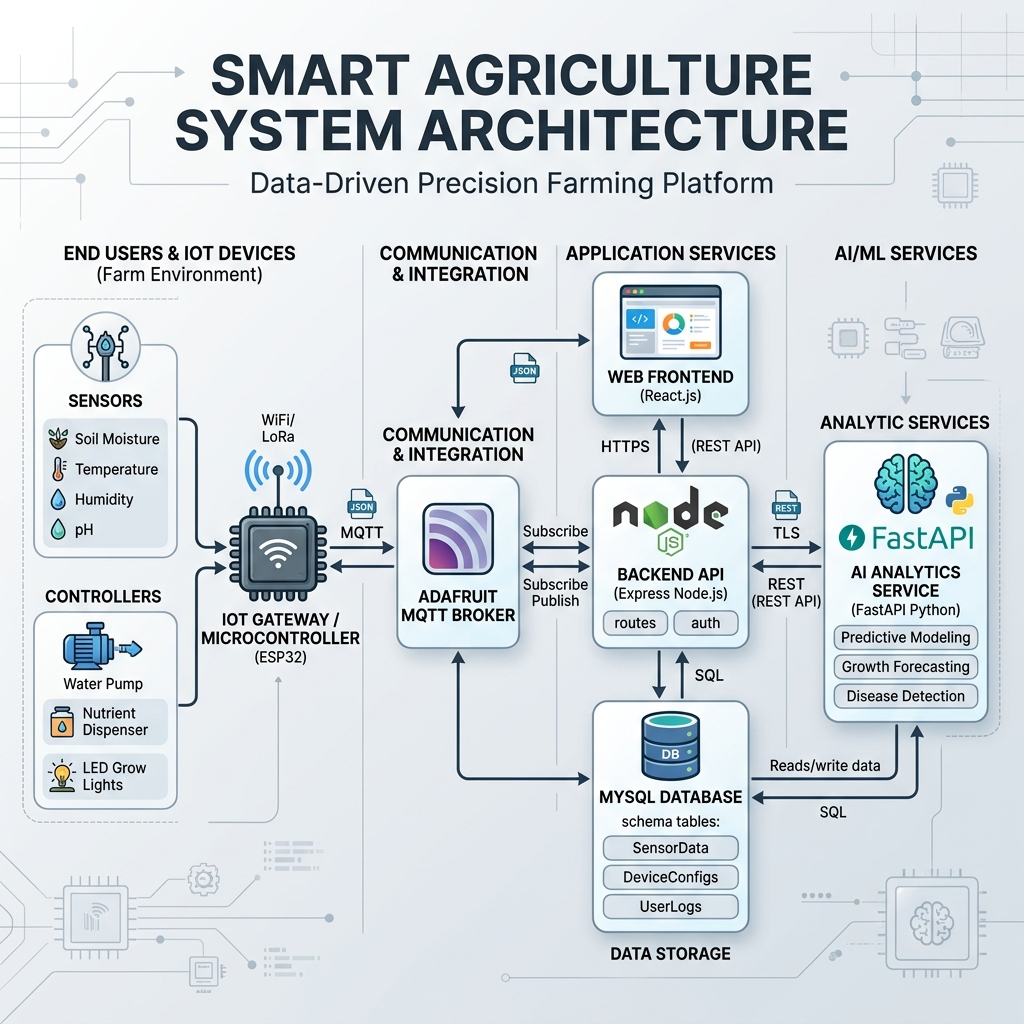
\includegraphics[width=0.75\linewidth]{./Pictures/Task_5/structure.png}
    \caption{Kiến trúc hệ thống SmartFarm}
\end{figure}

\begin{itemize}
    \item \textbf{Frontend}: React 19 + TypeScript + Vite
    \item \textbf{Backend}: Node.js + Express + Socket.IO
    \item \textbf{AI API}: FastAPI + TensorFlow/Keras (Python 3.10--3.12)
    \item \textbf{Database}: MySQL (mysql2)
    \item \textbf{IoT}: Adafruit IO (MQTT)
    \item \textbf{AI Model}: EfficientNet --- nhận diện 6 loại bệnh trên lá cà chua
\end{itemize}

\subsubsection{Tổng quan}
    \begin{longtable}{|P{0.35\linewidth}|m{0.58\linewidth}|}
        \hline
        \textbf{Tính năng} & \begin{center}\textbf{Mô tả}\end{center} \\
        \hline
        \textbf{Dashboard} & Giám sát cảm biến thời gian thực (nhiệt độ, độ ẩm, ánh sáng, độ ẩm đất) \\
        \hline
        \textbf{Điều khiển thiết bị} & Bật/tắt bơm nước, đèn LED, servo từ xa \\
        \hline
        \textbf{Lịch trình tưới tự động} & Lịch tưới theo ngày lặp lại, khoảng thời gian bắt đầu/kết thúc \\
        \hline
        \textbf{AI Phát hiện sâu bệnh} & Upload ảnh lá cây $\rightarrow$ mô hình AI nhận diện bệnh, trả về tên bệnh, giải pháp và độ tin cậy \\
        \hline
        \textbf{Thông báo} & Cảnh báo bất thường từ cảm biến và hệ thống, xóa từng thông báo hoặc xóa tất cả \\
        \hline
        \textbf{Quản lý người dùng} & Phân quyền admin/user, ban/unban, admin đổi tên/mật khẩu của bất kỳ user \\
        \hline
        \textbf{Hồ sơ cá nhân} & Đổi tên hiển thị, mật khẩu, upload avatar lên Cloudinary \\
        \hline
        \textbf{Cài đặt giao diện} & Theme sáng/tối, màu chủ đạo, font chữ, bo góc tùy chỉnh \\
        \hline
        \textbf{Chính sách bảo mật} & Admin quản lý nội dung policy; dịch tự động sang VI/EN qua Google Translate \\
        \hline
        \textbf{Đa ngôn ngữ} & Hỗ trợ Tiếng Việt và Tiếng Anh, chuyển đổi từ sidebar \\
        \hline
        \textbf{Google OAuth} & Đăng nhập bằng tài khoản Google \\
        \hline
        \caption{Các tính năng chính của hệ thống SmartFarm}
    \end{longtable}
    

\subsubsection{Giao diện đăng kí, đăng nhập}
\indent Để đảm bảo tính bảo mật và cá nhân hóa trải nghiệm người dùng, hệ thống yêu cầu người dùng phải có tài khoản phân quyền để truy cập vào trong hệ thống và điều khiển thiết bị.
\subsubsubsection{Giao diện đăng kí}
\indent Giao diện đăng kí cho phép người dùng mới tạo tài khoản bằng cách điền các thông tin cơ bản. Sau khi đăng kí thành công, tài khoản sẽ được lưu vào cơ sở dữ liệu MySQL và được cấp quyền người dùng cơ bản (user).
\begin{figure}[H]
	\centering
	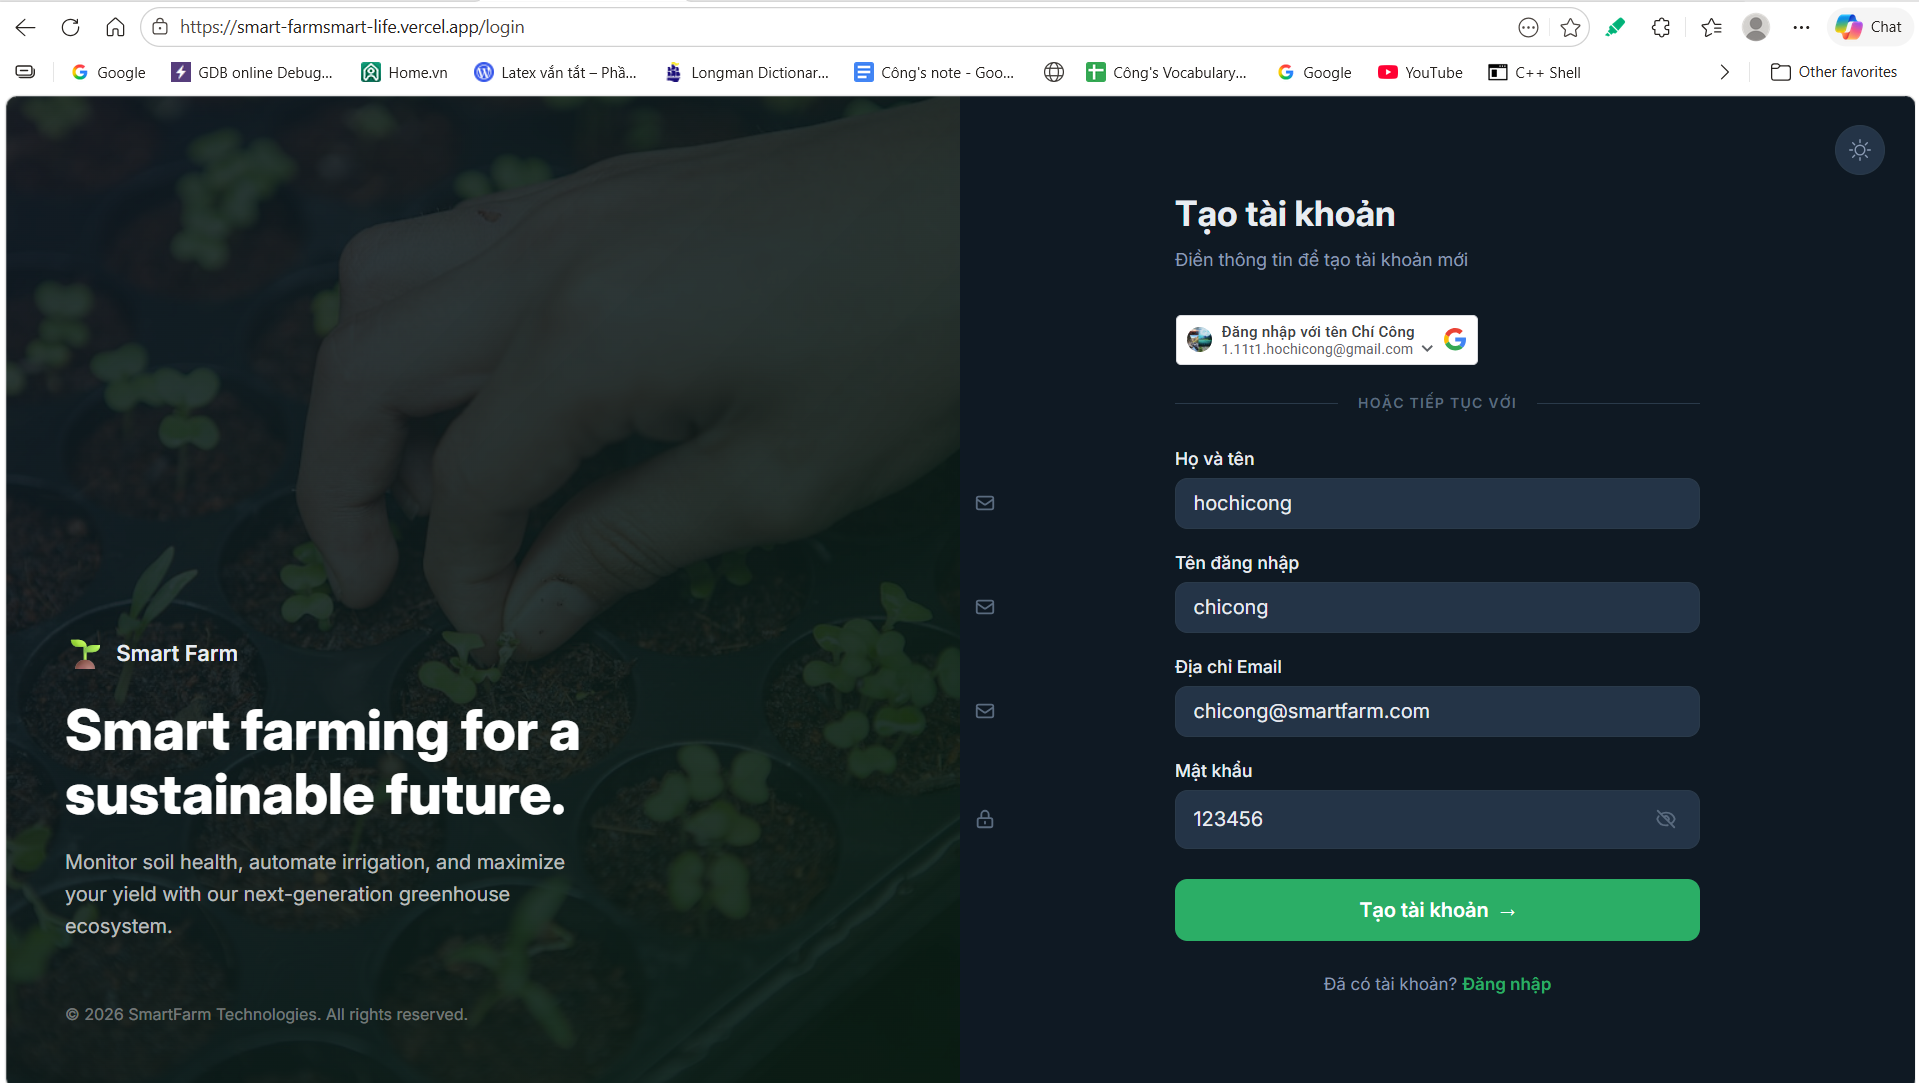
\includegraphics[width=0.8\linewidth]{./Pictures/Task_5/register.png}
	\caption{Giao diện đăng kí tài khoản mới}
\end{figure}

\subsubsubsection{Giao diện đăng nhập}
\indent Giao diện đăng nhập là điểm kết nối đầu tiên của người dùng, cung cấp các phương thức xác thực an toàn:
\begin{enumerate}[label=\textbf{\alph*.}]
	\item \textbf{Đăng nhập trực tiếp:} Người dùng điền tên đăng nhập và mật khẩu đã đăng kí. Hệ thống xử lý qua Node.js API và trả về JSON Web Token (JWT) để duy trì phiên đăng nhập.
	\begin{figure}[H]
		\centering
		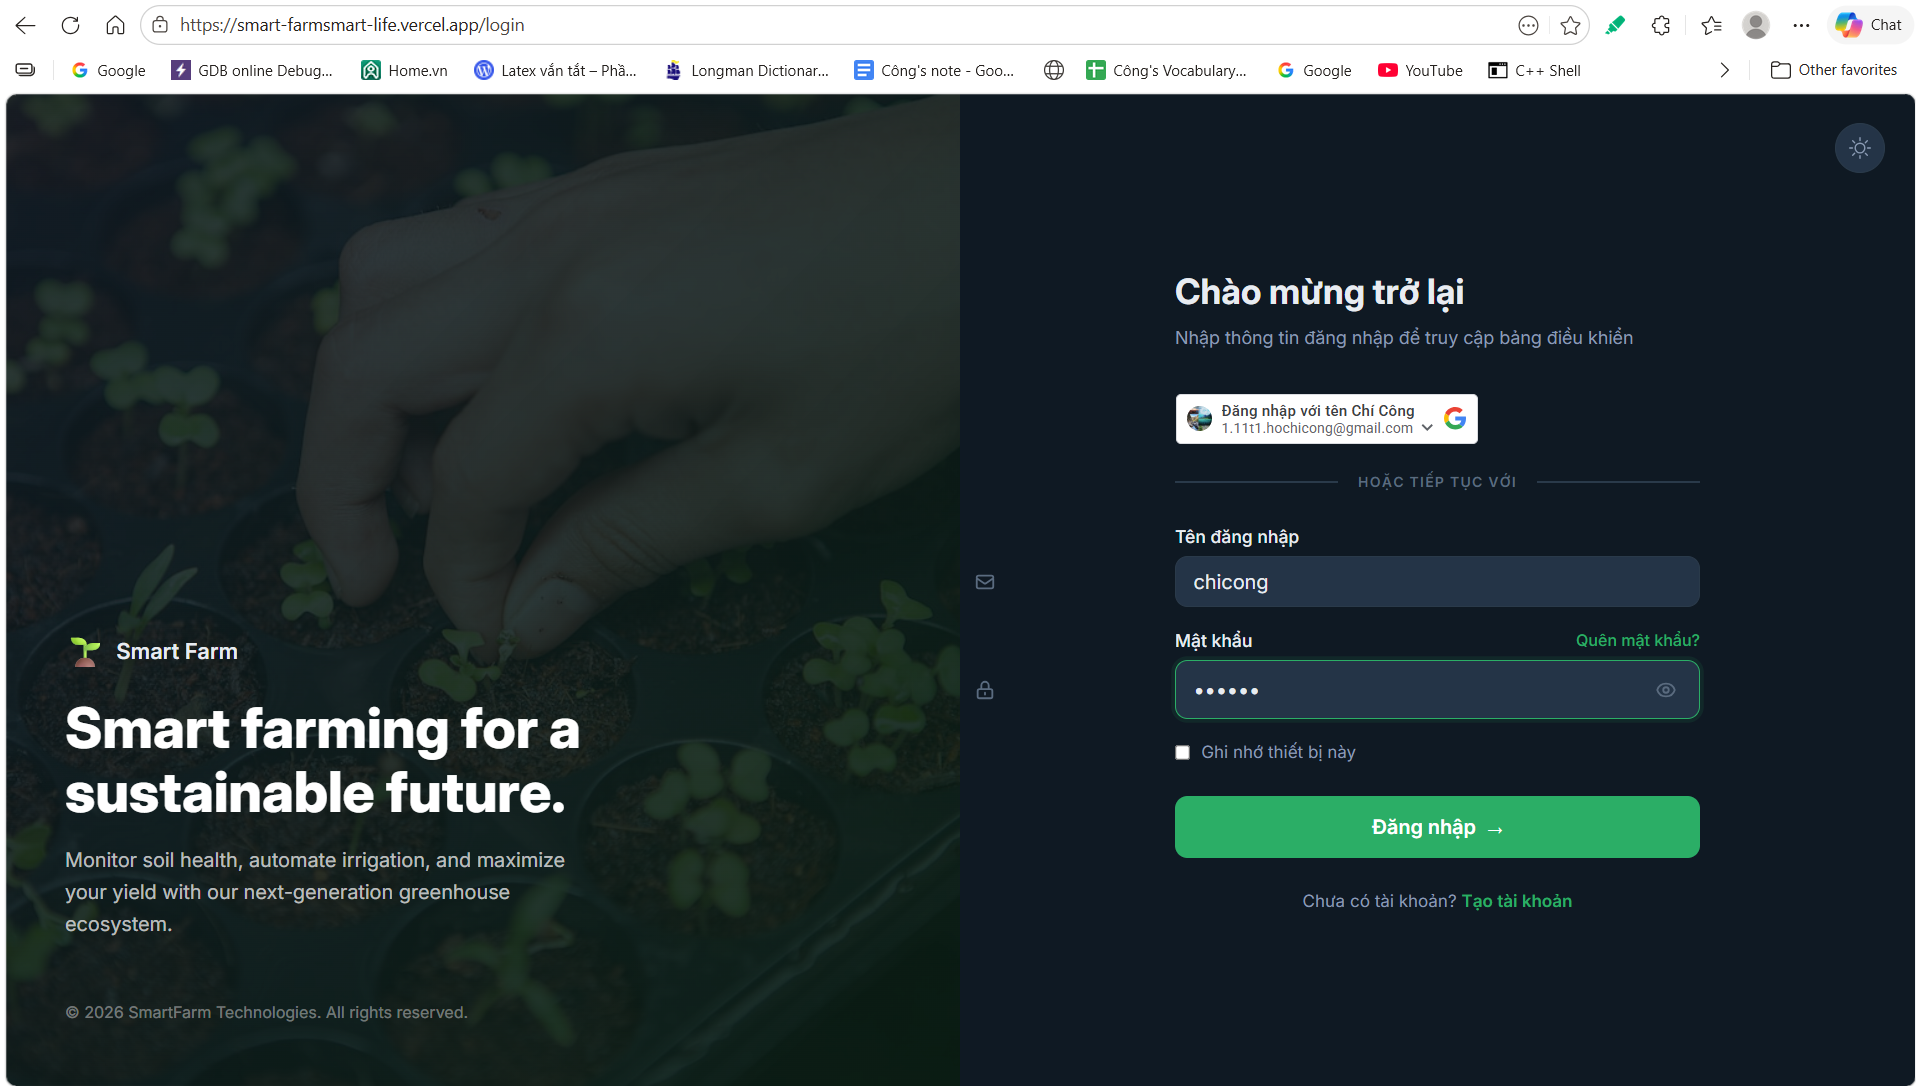
\includegraphics[width=0.8\linewidth]{./Pictures/Task_5/login_direct.png}
		\caption{Giao diện đăng nhập bằng tài khoản hệ thống}
	\end{figure}
	
	\item \textbf{Đăng nhập qua xác thực tài khoản Google (Google OAuth):} Hỗ trợ người dùng đăng nhập nhanh chóng và an toàn chỉ với một lần nhấn nhờ tích hợp Google OAuth 2.0, không cần nhớ mật khẩu riêng cho hệ thống.
	\begin{figure}[H]
		\centering
		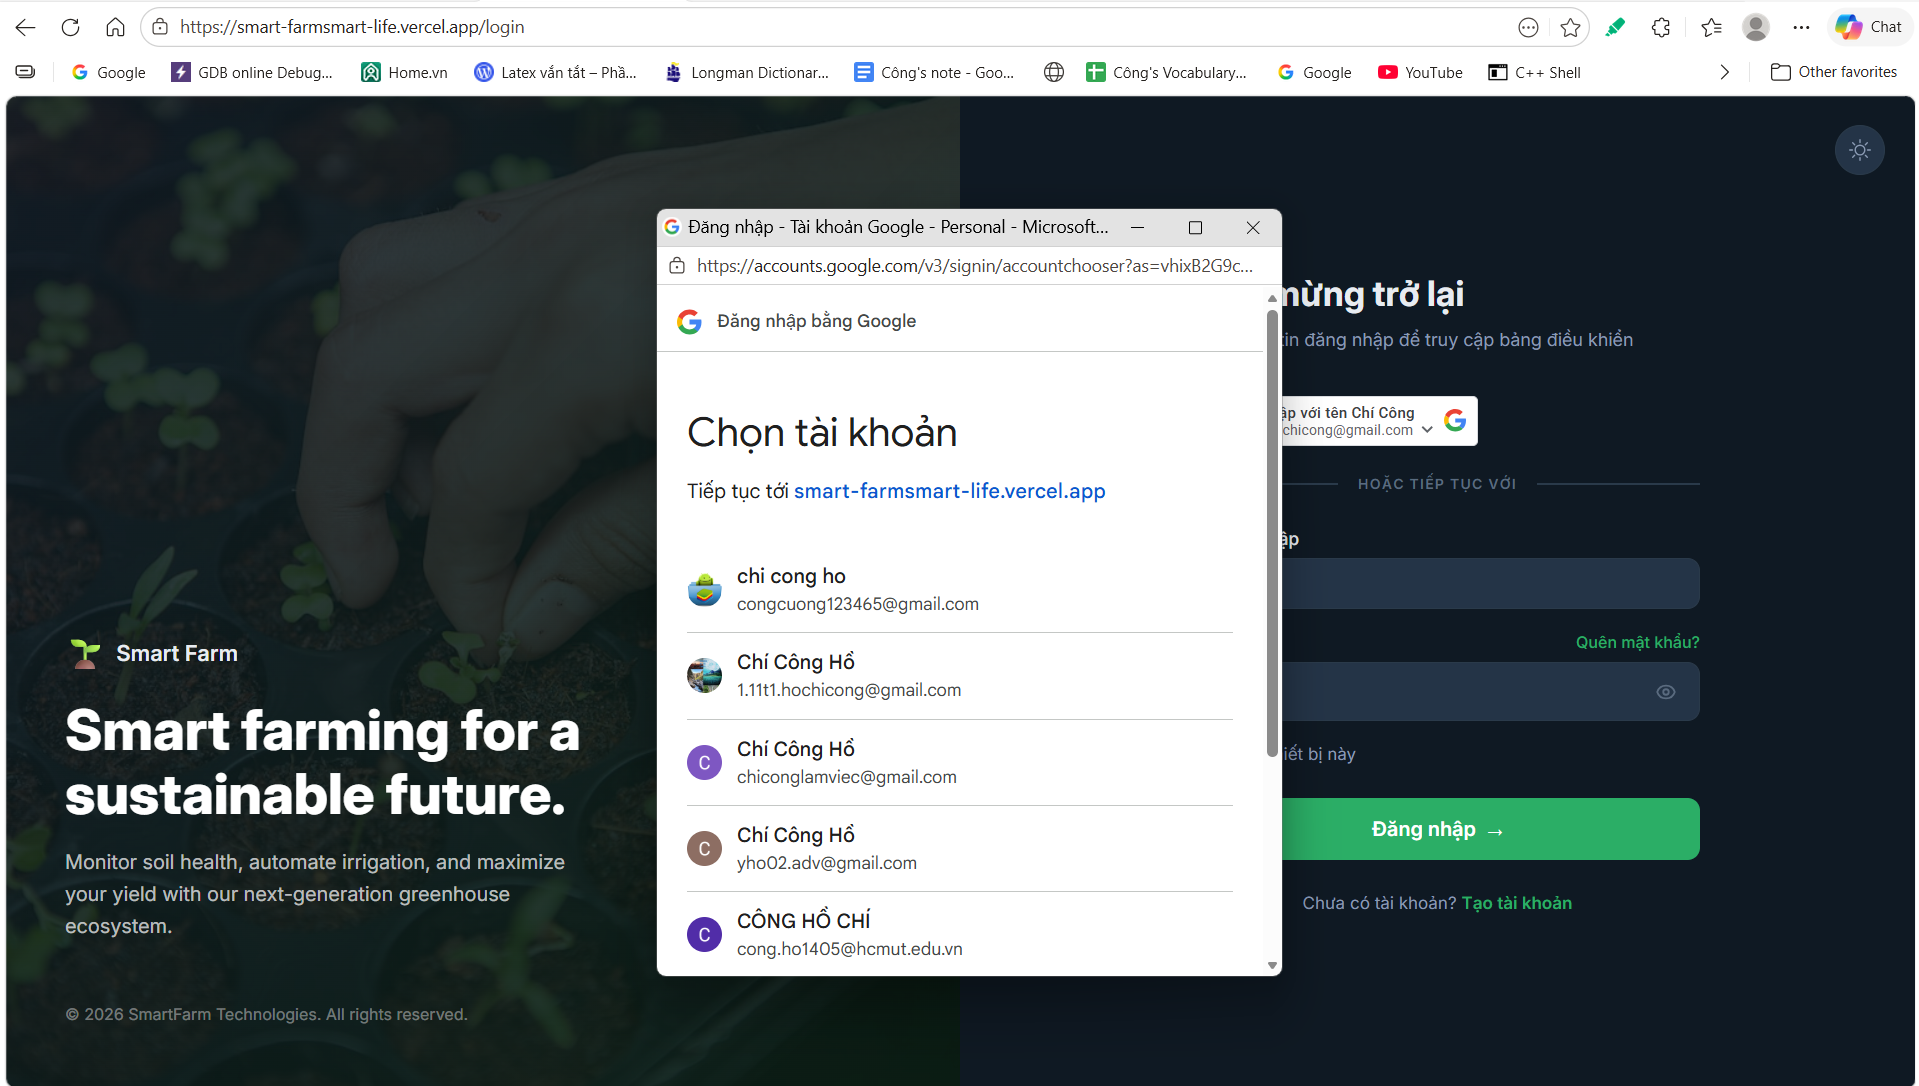
\includegraphics[width=0.8\linewidth]{./Pictures/Task_5/login_google.png}
		\caption{Giao diện đăng nhập thông qua Google OAuth}
	\end{figure}
\end{enumerate}
\subsubsection{Giao diện phần cài đặt của hệ thống}
\indent Giao diện cài đặt cung cấp trung tâm để cá nhân hóa và quản trị trang web. Trang này gồm nhiều thẻ chức năng khác nhau:
\begin{enumerate}[label=\textbf{\alph*.}]
	\item \textbf{Tùy chỉnh giao diện trang web:} Hiện tại, hệ thống hỗ trợ hai ngôn ngữ, đó là Tiếng Anh và Tiếng Việt. Phần dịch thuật song song hai ngôn ngữ này được tiến hành dựa vào kiến trúc i18n. Ngoài ra, người dùng có thể tùy ý thay đổi theme (sáng/tối), màu sắc chủ đạo, font chữ và độ bo góc của các thành phần giao diện. Các thông số này sẽ được lưu lại để tự động áp dụng trong các lần tiếp theo.
	\begin{figure}[H]
		\centering
		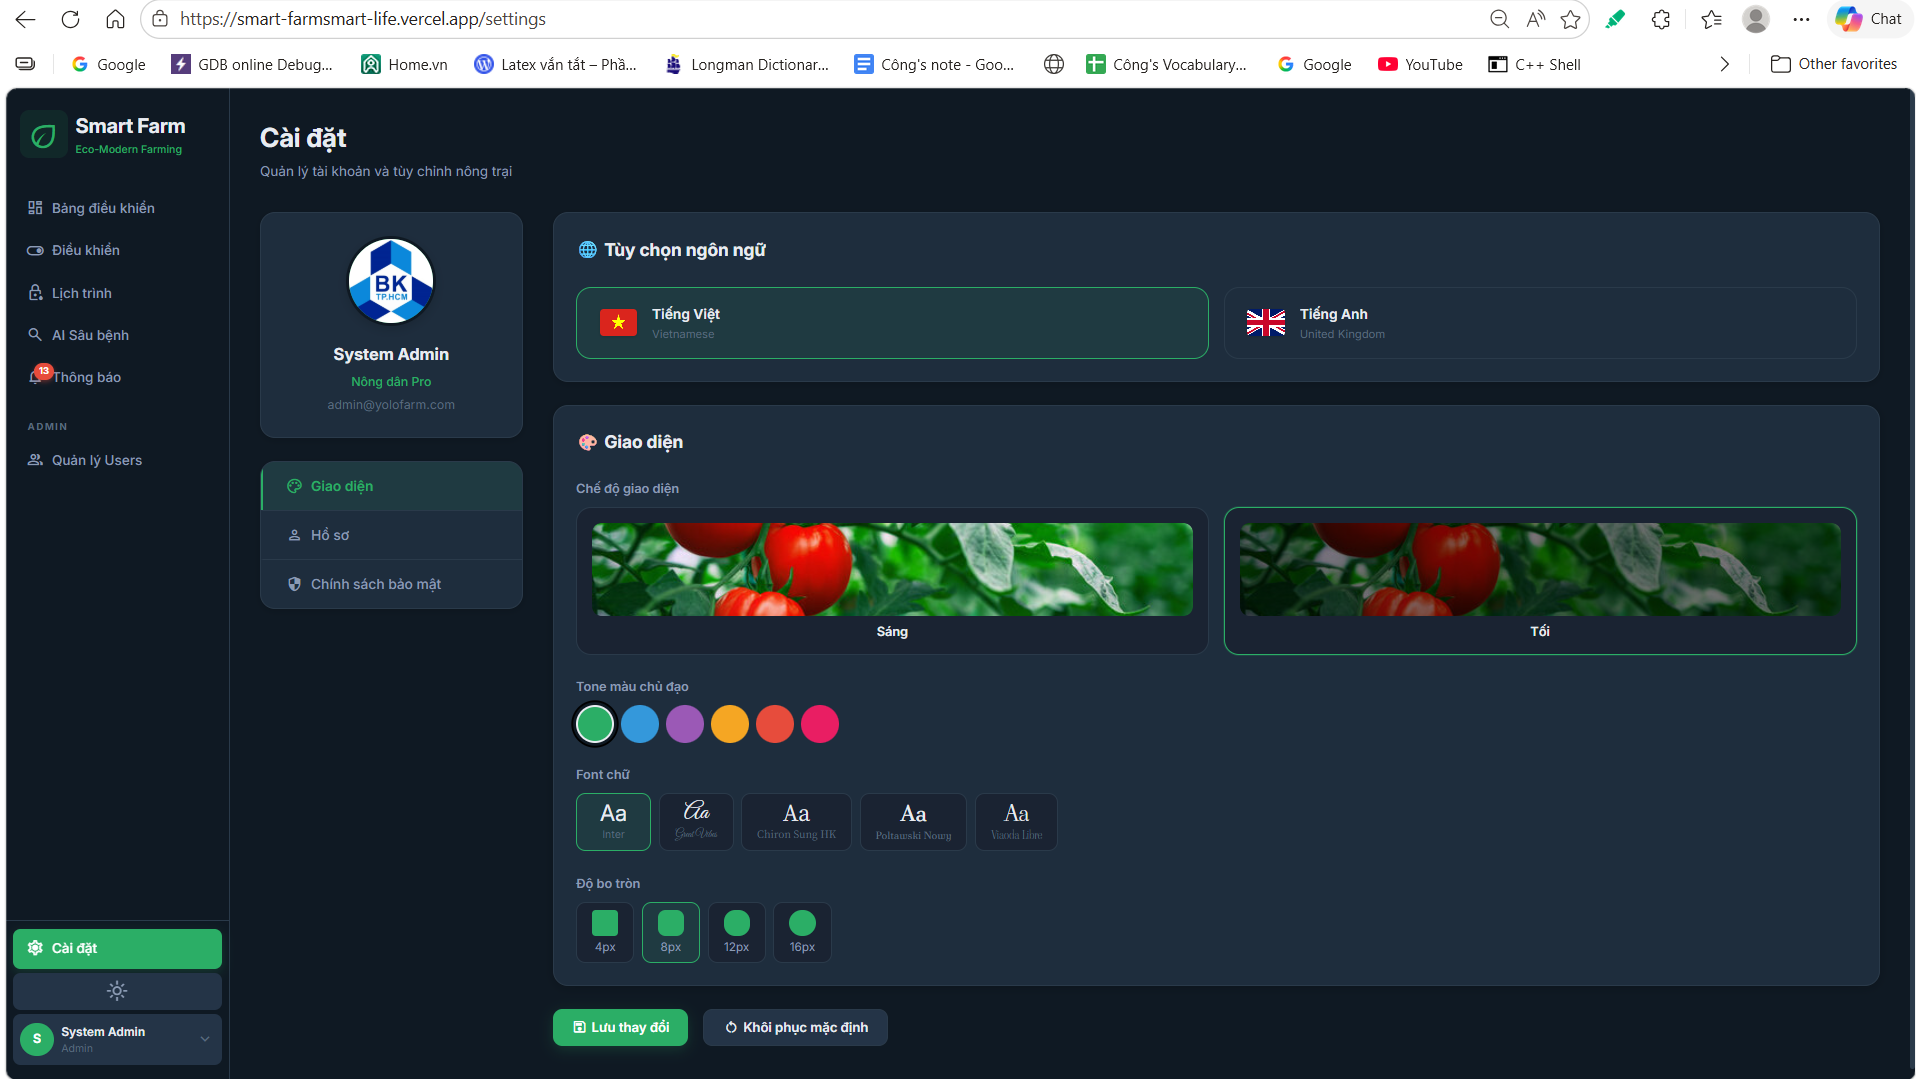
\includegraphics[width=0.85\linewidth]{./Pictures/Task_5/setting_preference.png}
		\caption{Tùy chỉnh giao diện trang web}
	\end{figure}
	
	\item \textbf{Xem hồ sơ của bản thân:} Nơi người dùng có thể cập nhật thông tin cá nhân bao gồm thay đổi tên hiển thị, thay đổi mật khẩu. Cụ thể, việc đổi mật khẩu chỉ có thể được thực hiện bởi người dùng đăng nhập vào hệ thống trực tiếp thay vì đăng nhập bằng tài khoản Google. Nếu đăng nhập bằng tài khoản Google thì người dùng đó không thể điều chỉnh được mật khẩu Google của mình qua trang web này. Đặc biệt, người dùng có thể tải lên ảnh đại diện (avatar) cá nhân, hệ thống sẽ sử dụng dịch vụ Cloudinary để lưu trữ ảnh an toàn.
	\begin{figure}[H]
		\centering
		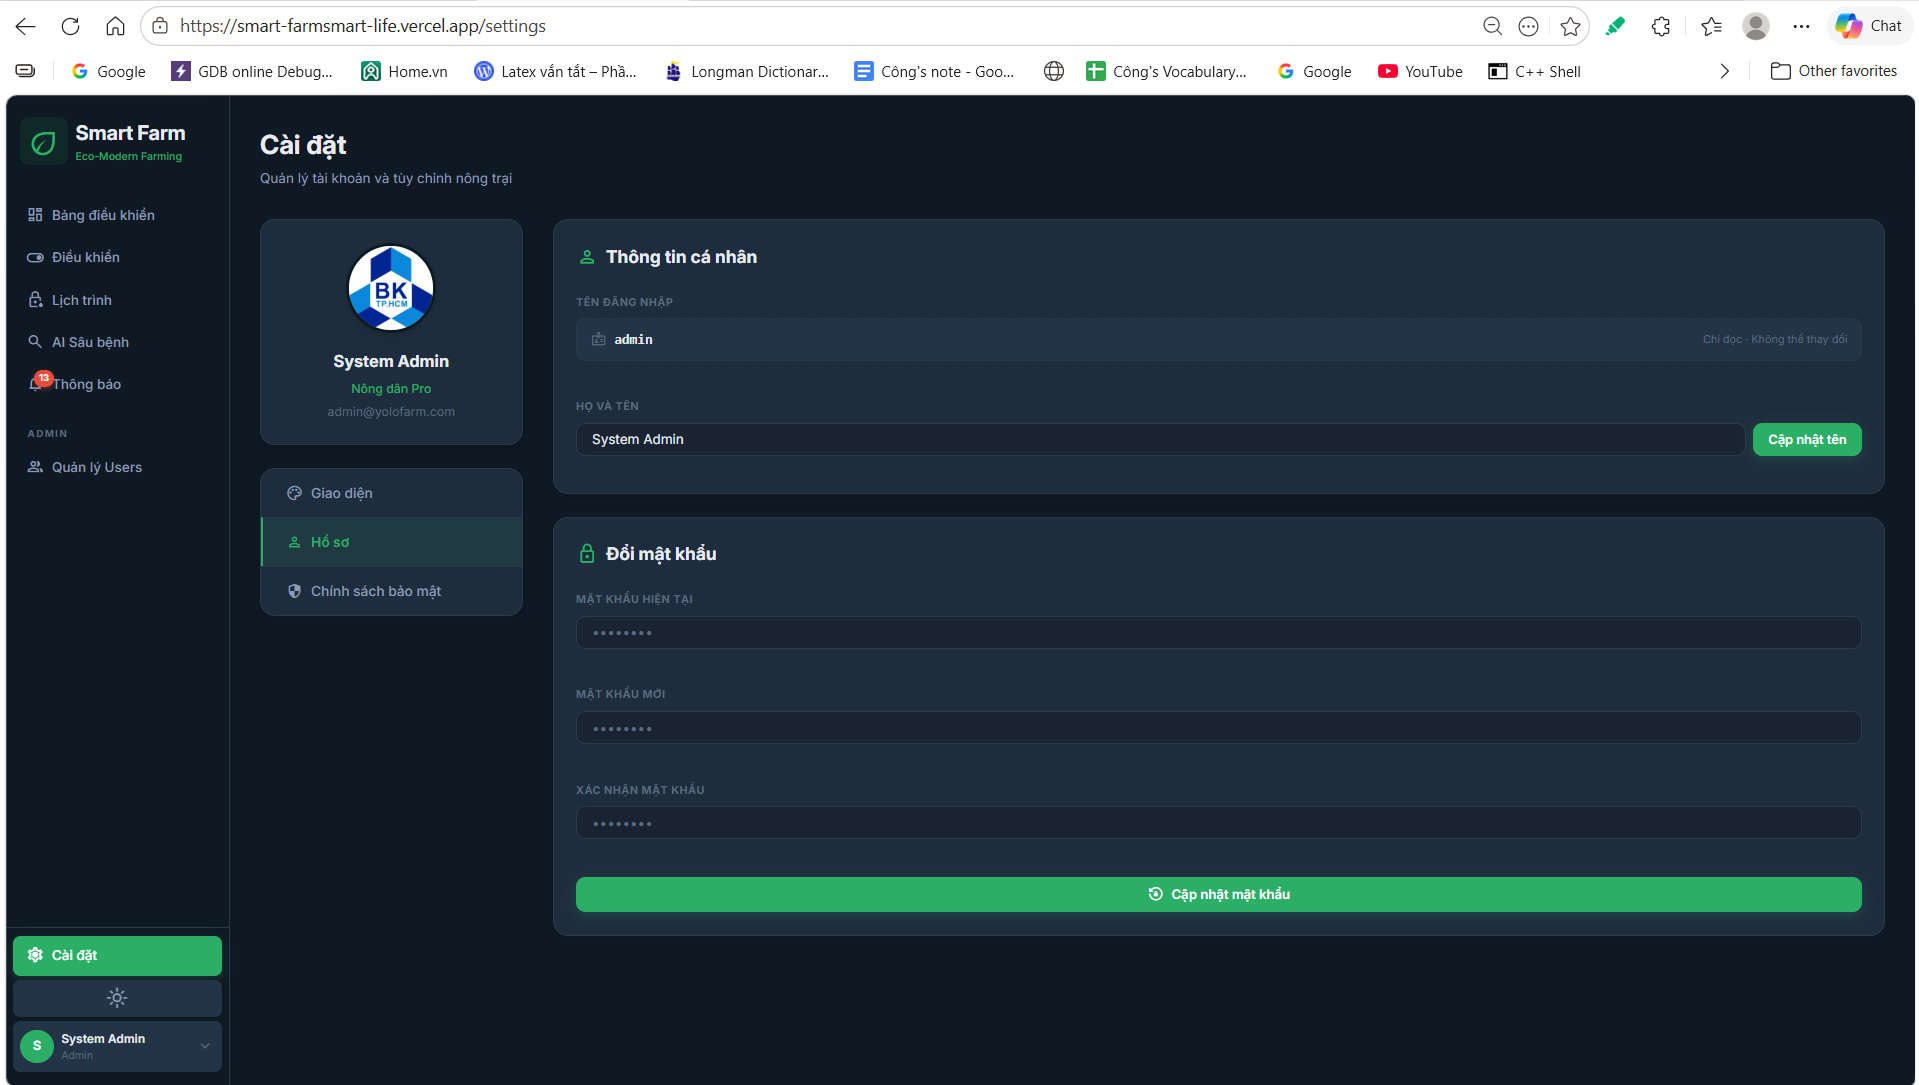
\includegraphics[width=0.85\linewidth]{./Pictures/Task_5/setting_profile.png}
		\caption{Quản lý hồ sơ cá nhân}
	\end{figure}
	
	\item \textbf{Xem chính sách bảo mật của hệ thống:} Hiển thị rõ ràng các quy định sử dụng và chính sách bảo vệ dữ liệu theo dạng Markdown preview.
	\begin{figure}[H]
		\centering
		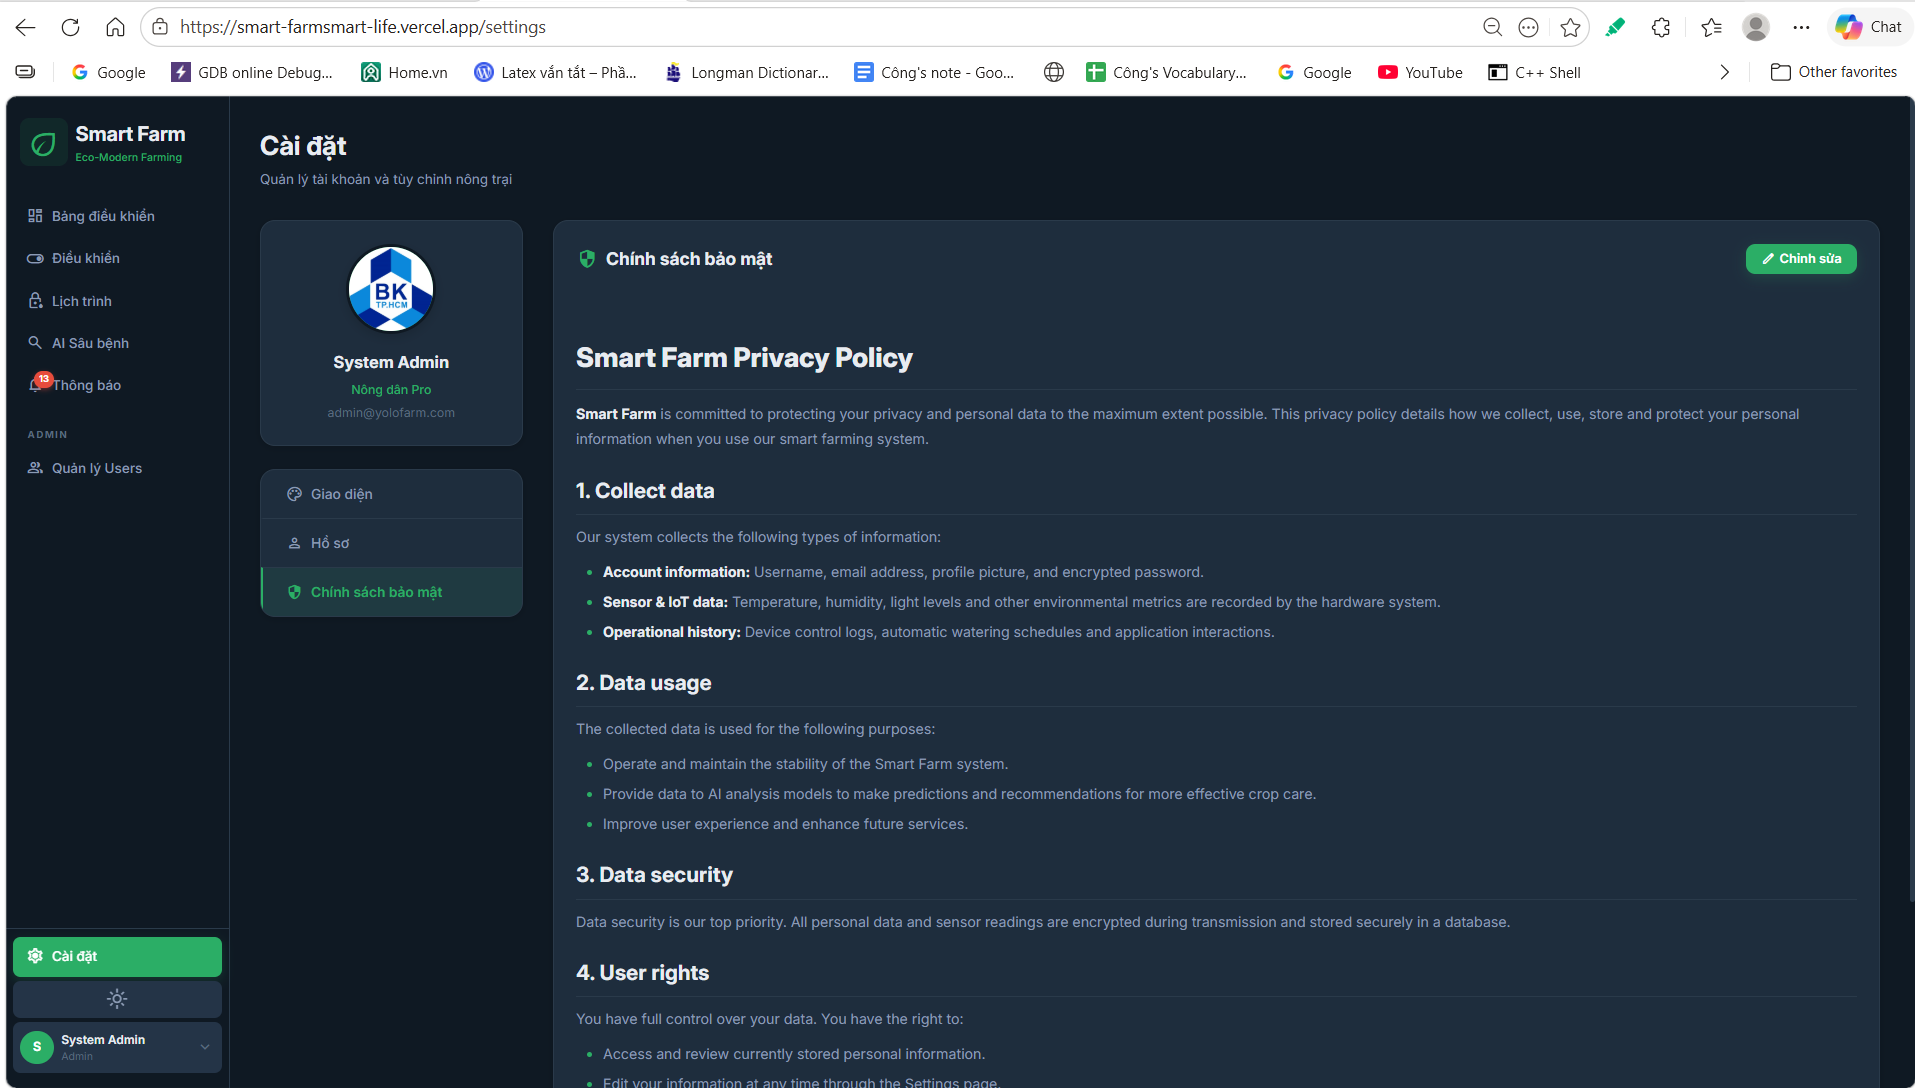
\includegraphics[width=0.85\linewidth]{./Pictures/Task_5/setting_policy.png}
		\caption{Giao diện hiển thị Chính sách bảo mật}
	\end{figure}
	
	\item \textbf{Admin tạo chính sách bảo mật:} Chức năng đặc quyền dành riêng cho quản trị viên (Admin). Admin có thể thêm, chỉnh sửa hoặc xóa nội dung các chính sách của website một cách trực tiếp từ giao diện văn bản bằng cách sử dụng định dạng markdown.
	\begin{figure}[H]
		\centering
		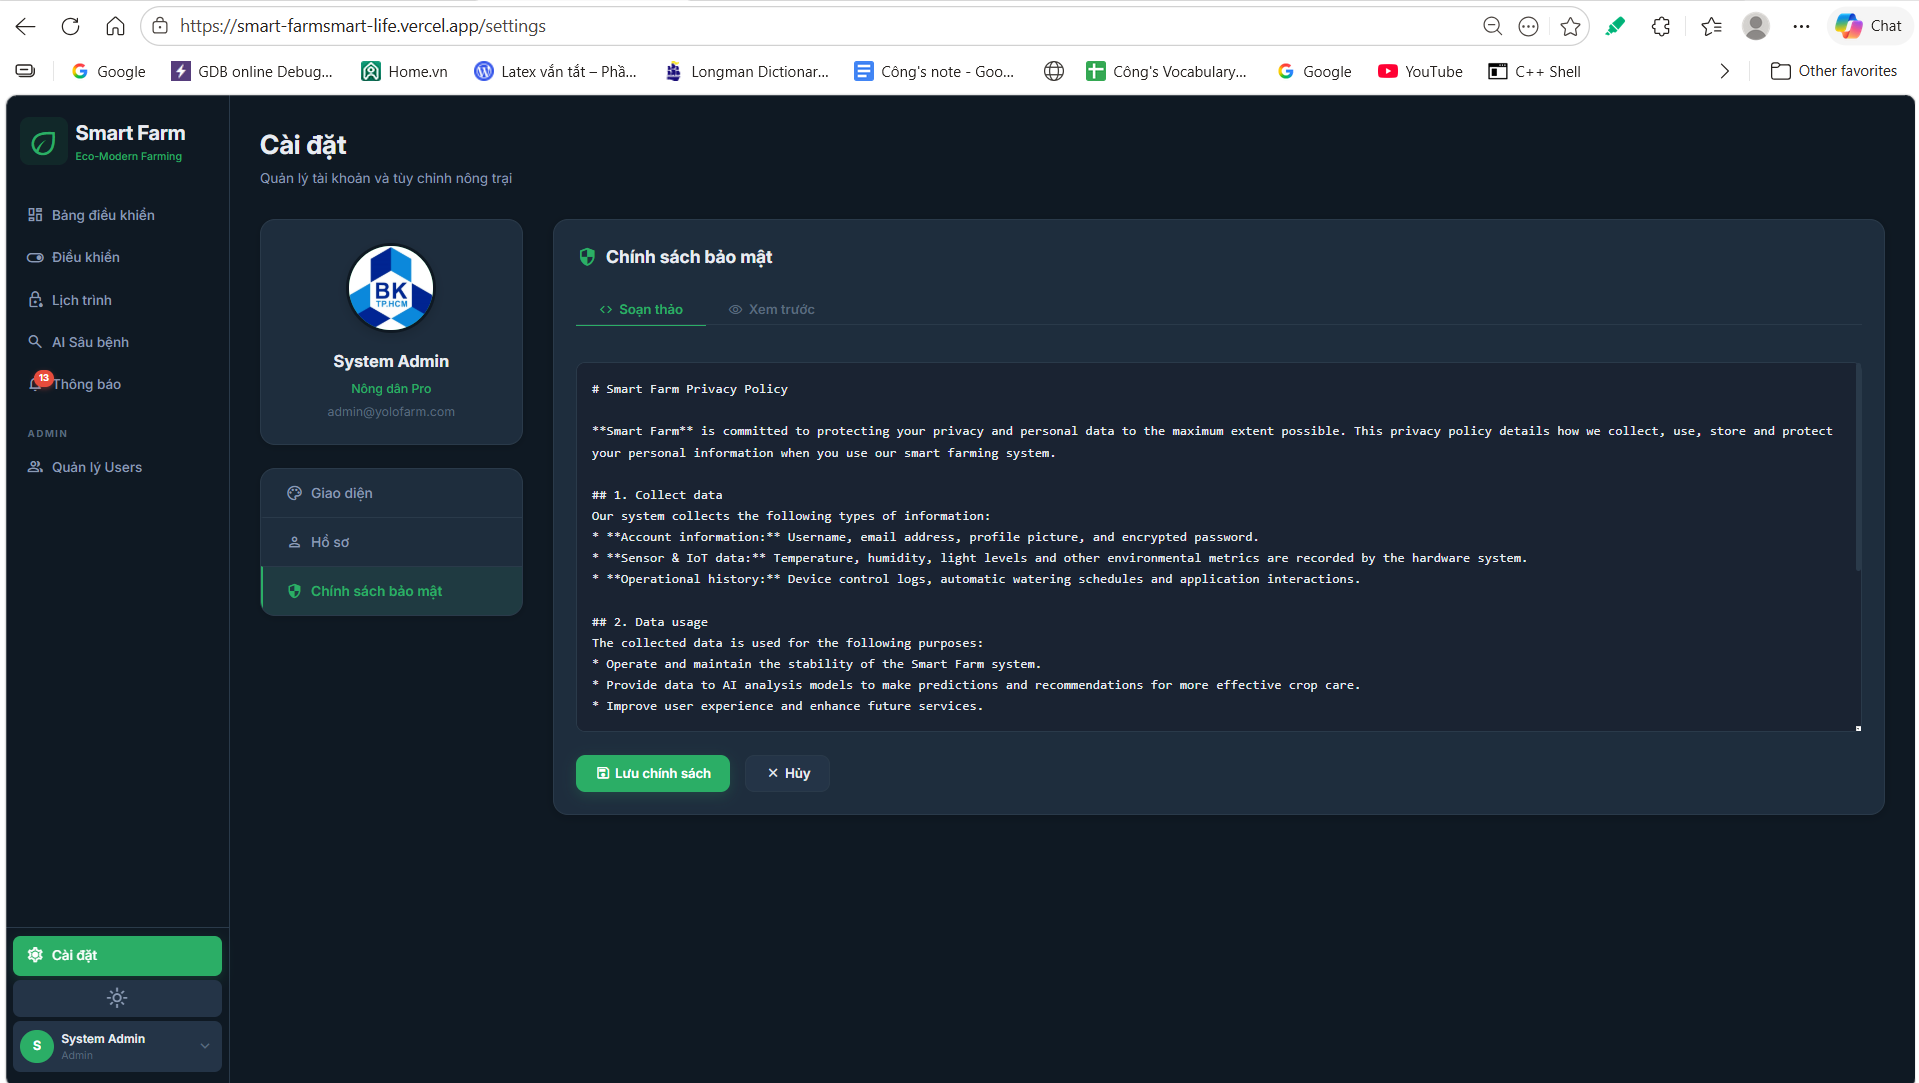
\includegraphics[width=0.85\linewidth]{./Pictures/Task_5/setting_policy_admin.png}
		\caption{Giao diện quản lý Chính sách bảo mật cho quản trị viên}
	\end{figure}

	\item \textbf{Quản lý người dùng (Dành cho Admin):} Phân quyền quản trị cho phép Admin xem danh sách tất cả tài khoản, thực hiện các thao tác cấm (ban) hoặc bỏ cấm (unban) những người dùng có hành vi sai phạm. Ngoài ra cũng có thể thay đổi mật khẩu của một tài khoản user bất kỳ. Khi thay đổi mật khẩu của một người dùng thì hệ thống sẽ gửi mật khẩu mới cho người dùng đó thông qua mục thông báo. Mặt khác, admin cũng có thể thay đổi vai trò của các người dùng khác thành admin hoặc ngược lại.
	\begin{figure}[H]
		\centering
		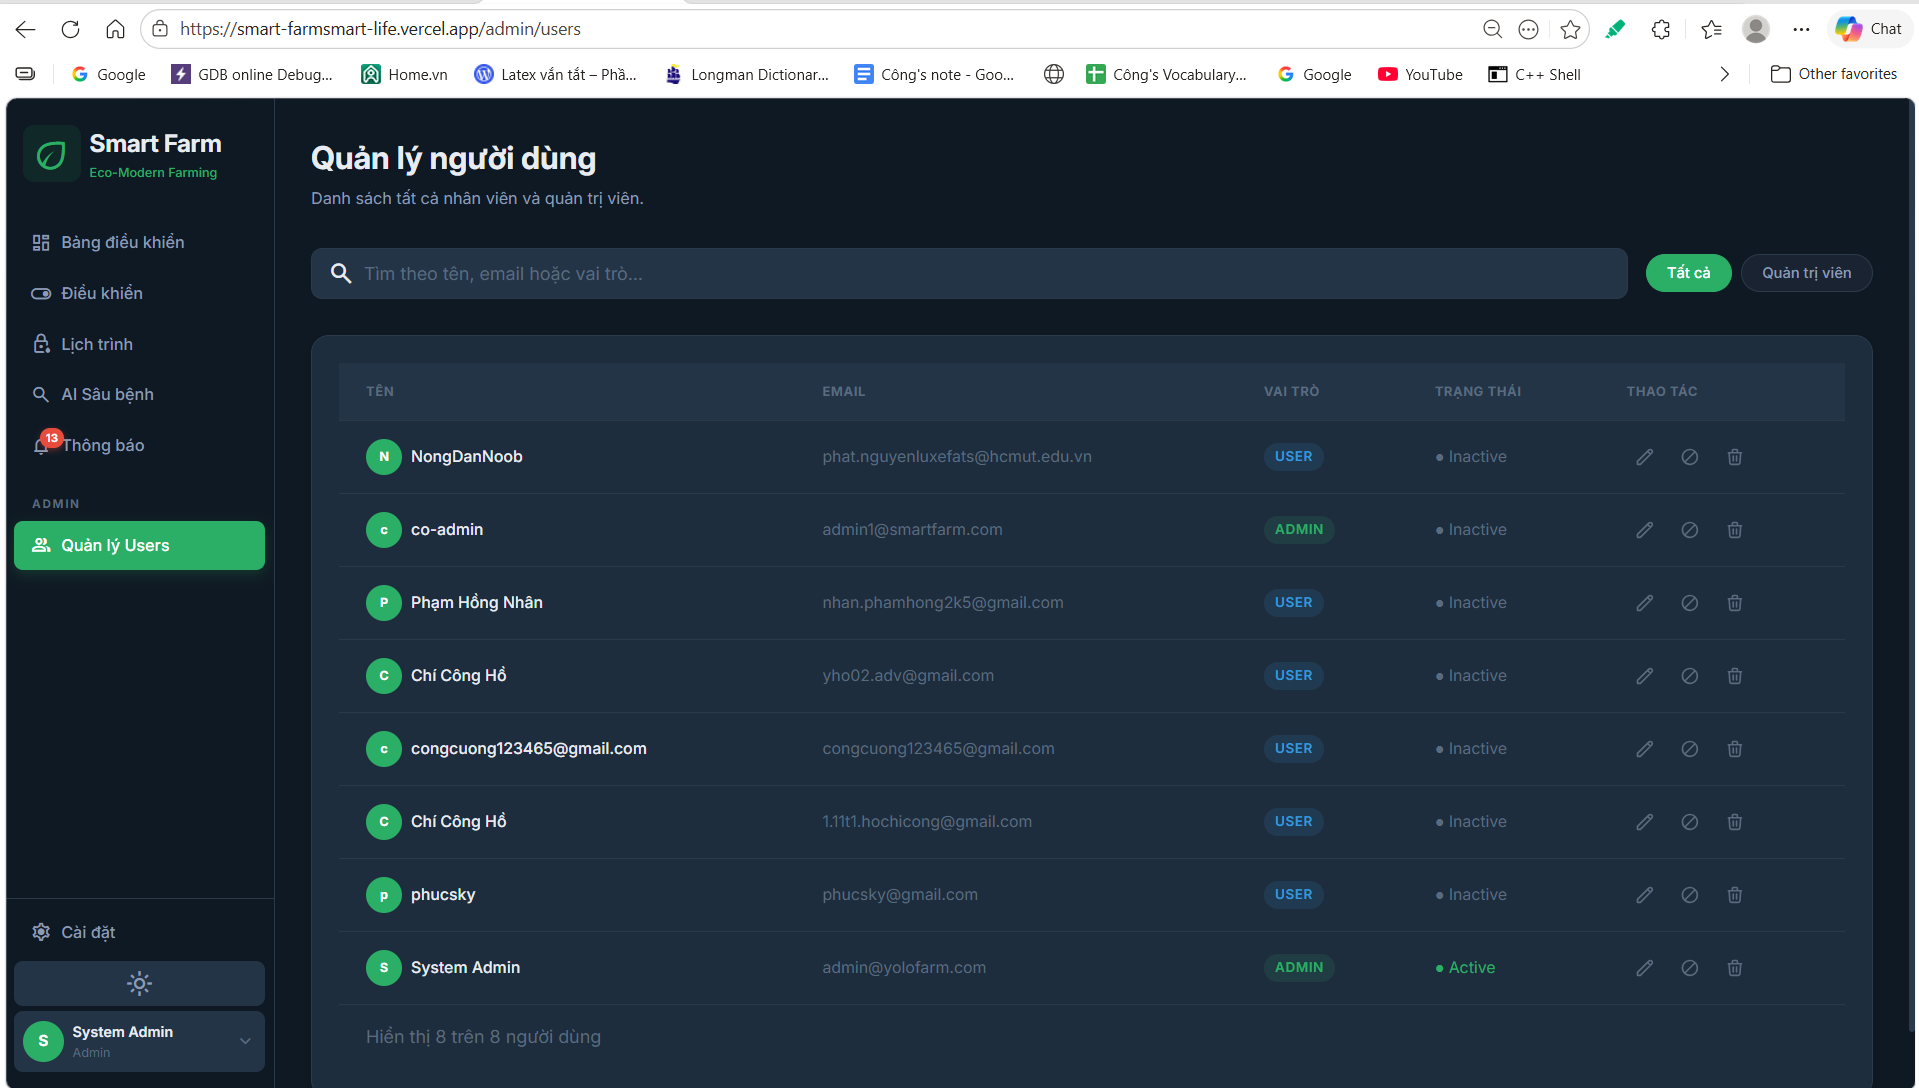
\includegraphics[width=0.85\linewidth]{./Pictures/Task_5/admin_manage_user.png}
		\caption{Danh sách Quản lý người dùng tập trung của Admin}
	\end{figure}
\end{enumerate}
\subsubsection{Giao diện Dashboard}
\indent Phần giao diện tổng quan của hệ thống gồm có 3 phần chính:
\begin{enumerate}[label=\arabic*., leftmargin=1.5cm]
    \item Phần xem nhiệt độ, độ ẩm, độ ẩm đất: Thông tin của các cảm biến được hiển thị dưới dạng số liệu được lấy từ adafruit-io. Số liệu được đưa lên adafruit chính là số liệu thật của các cảm biến tương ứng trả về. Cụ thể hơn, nếu chưa có phần cứng trực tiếp kết nối với adafruit thì hệ thống sẽ gọi API tới open-meteo để lấy dữ liệu thời tiết thật tại tọa độ xác định và gửi dữ liệu lên Adafruit. Đảm bảo rằng dữ liệu luôn được cập nhật một cách chính xác.
    \item Phần điều khiển thiết bị: Người dùng có thể điều khiển các thiết bị như hai máy bơm nước và đèn LED từ xa (có thể điều khiển từ các thiết bị khác nhau) nhờ việc đã kết nối hệ thống phần mềm với Adafruit và đồng thời kết nối Adafruit với hệ thống phần cứng. Điều này cho phép rằng, một khi phần mềm được deploy thành công, tức có nhiều người dùng truy cập vào hệ thống cùng một lúc thì có thể cùng điều khiển các thiết bị có trong nông trại.
    \item Phần biểu đồ miền hiển thị thông tin lịch sử nhiệt độ, độ ẩm, độ ẩm đất và cường độ ánh sáng mà các cảm biến ghi nhận được trong một ngày. Cụ thể, hệ thống sẽ lấy dữ liệu trực tiếp tại adafruit, tổng hợp lại và vẽ điểm tương ứng ra phần biểu đồ miền này. Từ đó giúp cho việc huấn luyện mô hình dự đoán xu hướng thời tiết, độ ẩm, cường độ ánh sáng và giúp xác định loại bệnh của lá cây một cách dễ dàng hơn.
\end{enumerate}
\begin{figure}[H]
	\centering
	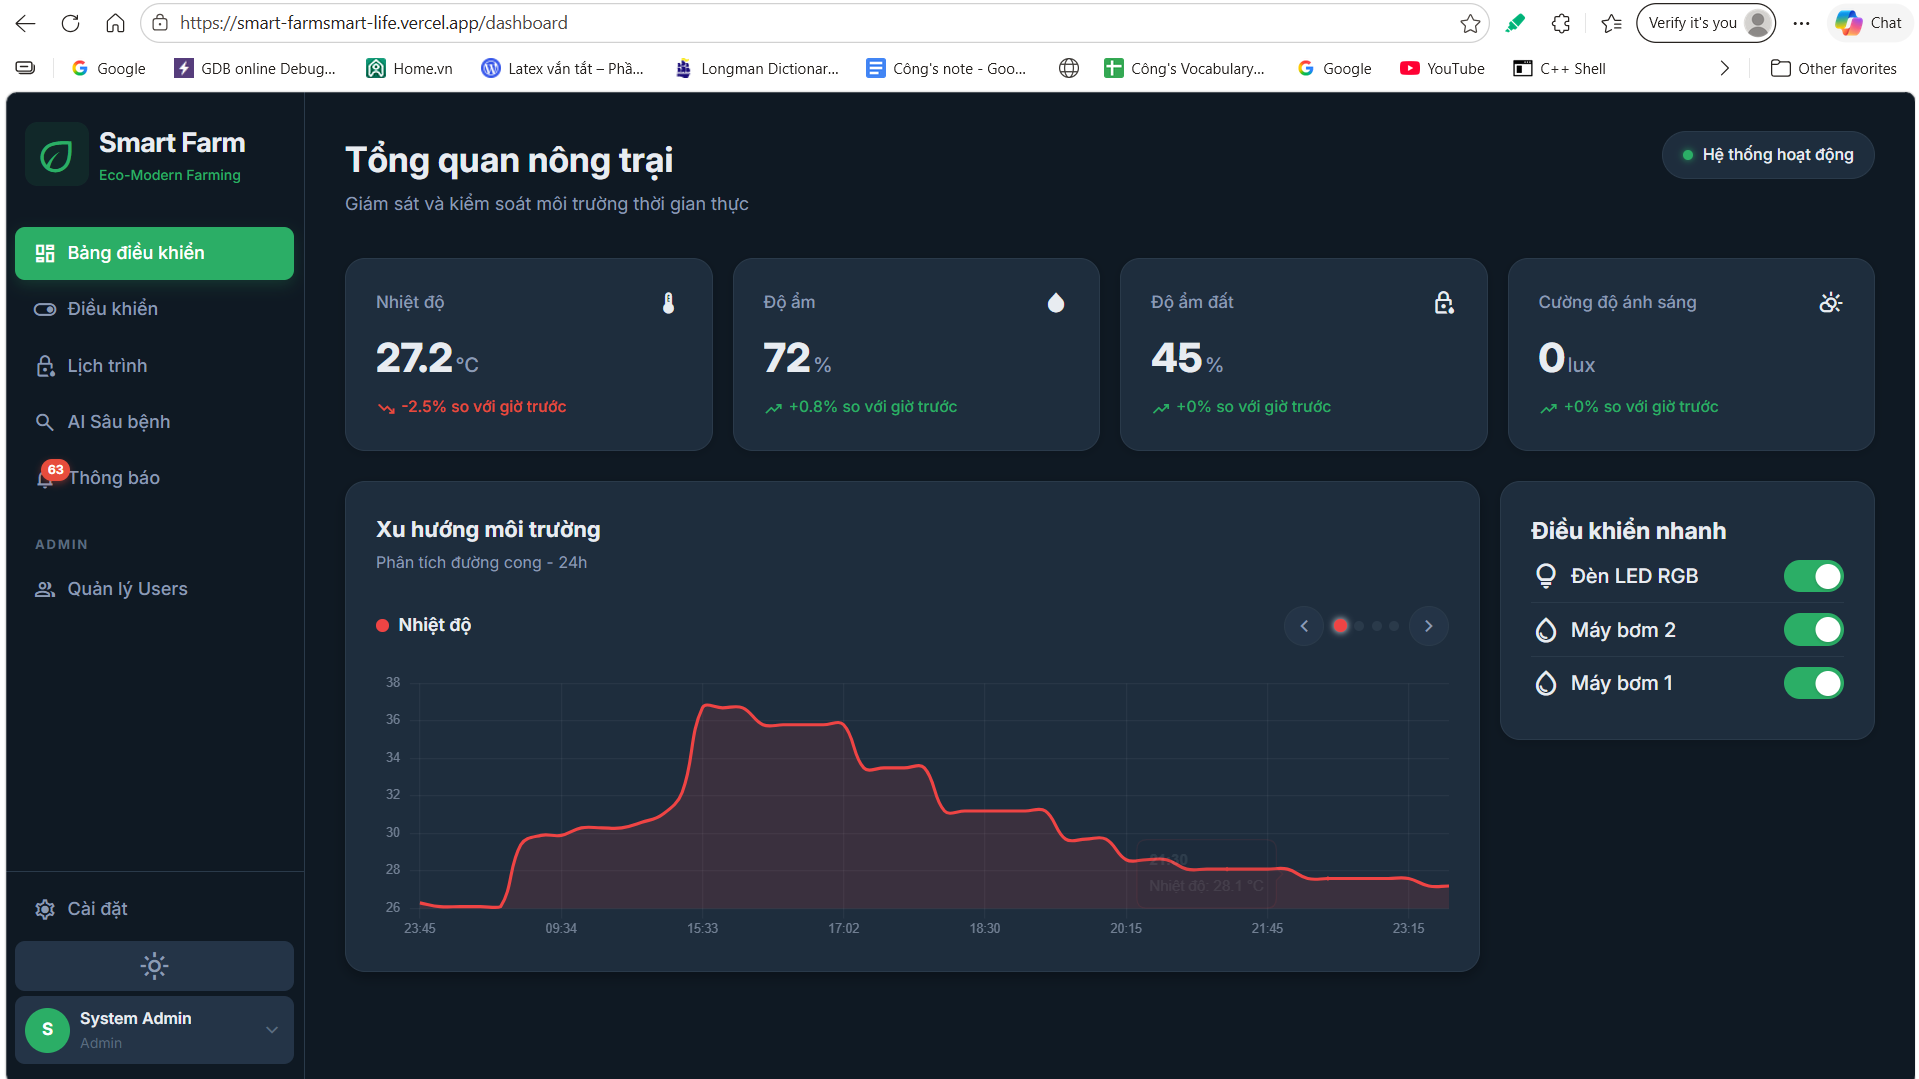
\includegraphics[width=0.8\linewidth]{./Pictures/Task_5/overview.png}
	\caption{Tổng quan hệ thống}
\end{figure}
\subsubsection{Giao diện điều khiển}
\indent Giao diện điều khiển là nơi cho phép người dùng quản lý trọn vẹn tất cả thiết bị được kết nối. Khi người dùng thao tác tương tác bằng cách bật/tắt thiết bị tại đây, tín hiệu sẽ đi qua backend API viết trên Node.js và nhanh chóng giao tiếp với Adafruit IO trực tiếp thông qua giao thức MQTT.\\
\indent Hệ thống hỗ trợ xử lý nhiều thiết bị cùng lúc (ví dụ như hai máy bơm \texttt{pump1}, \texttt{pump2} và một đèn \texttt{led-rgb}). Các trạng thái đang hoạt động, khu vực được phân bổ, chức năng, và thời gian hoạt động của máy bơm nước hay đèn chiếu sáng đều được phản hồi theo thời gian thực (realtime) lên phần mềm. Điều này có nghĩa là cho dù thiết bị được bật, tắt từ web app, hay từ mạng phần cứng, trạng thái đều đồng bộ cả hai chiều, giúp người dùng dễ quản lý và hạn chế rủi ro cho trang trại.
\begin{figure}[H]
	\centering
	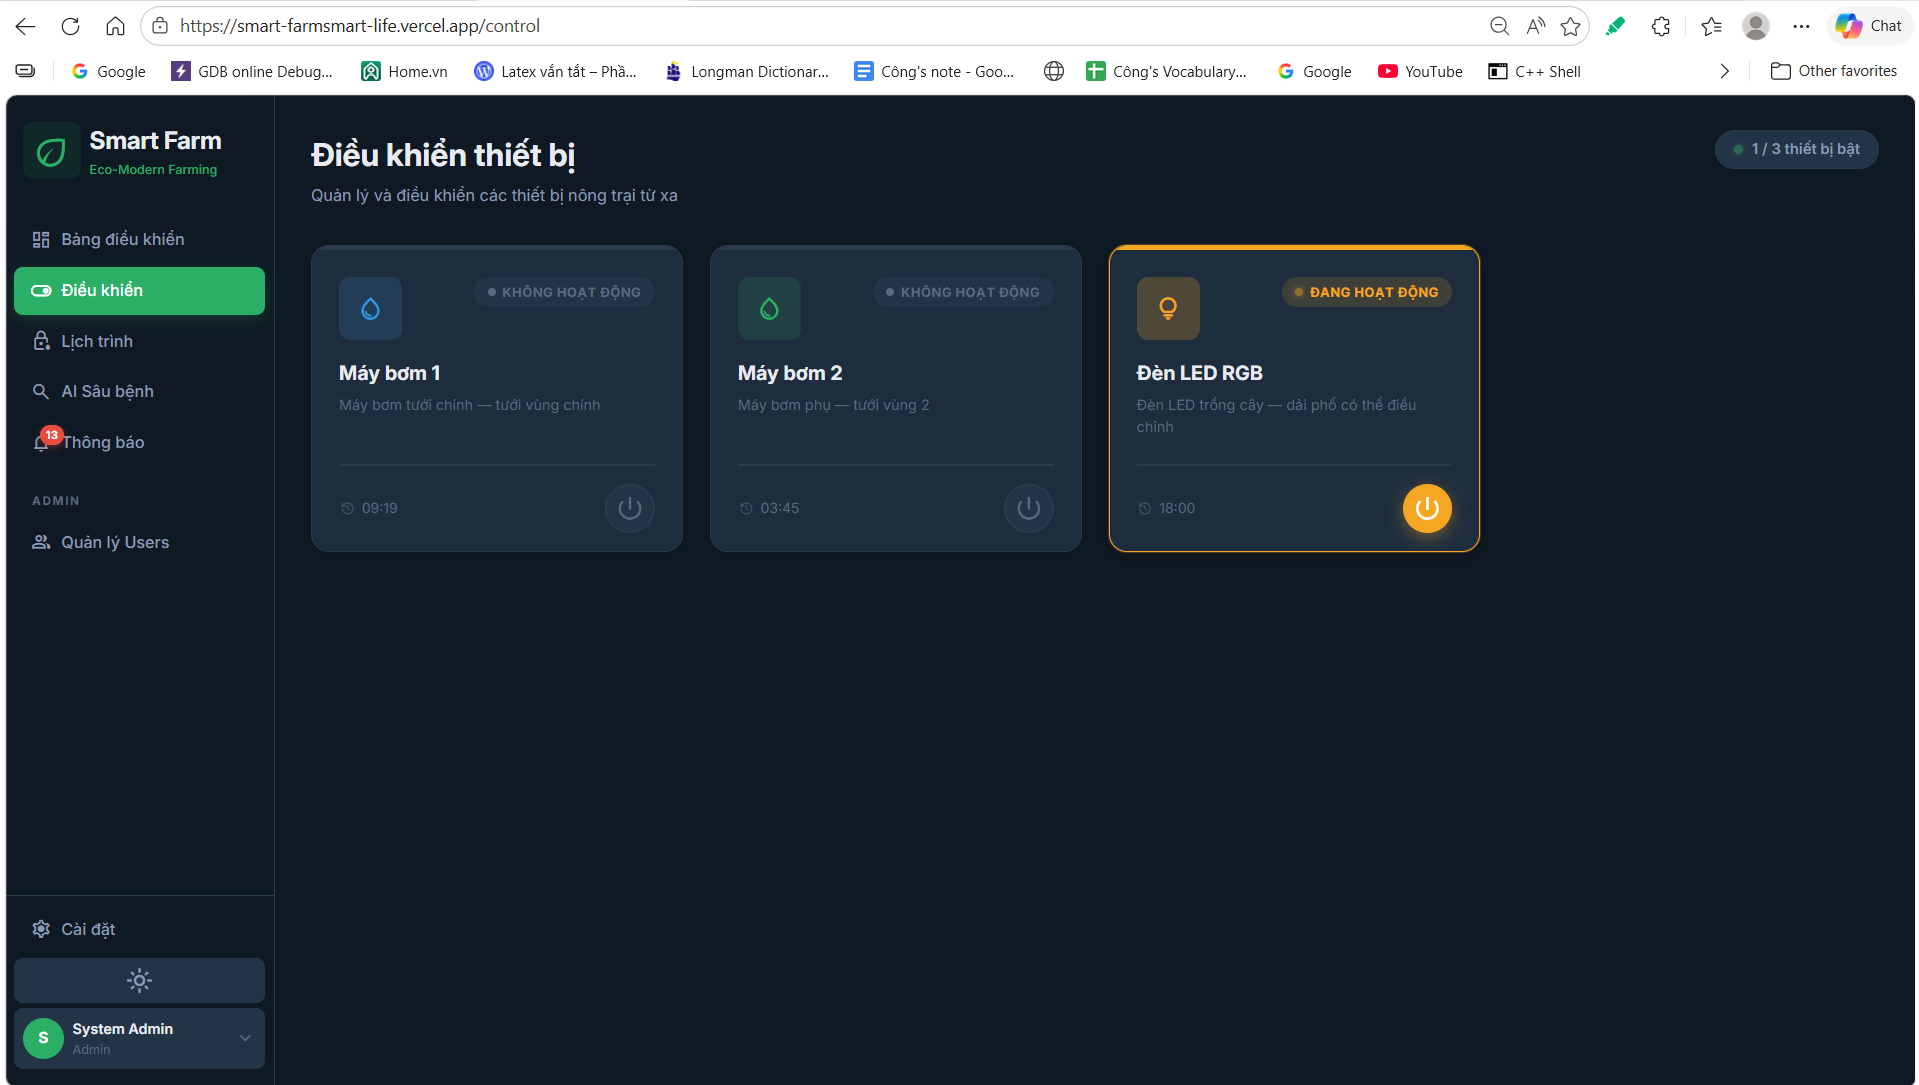
\includegraphics[width=0.8\linewidth]{./Pictures/Task_5/control_panel.png}
	\caption{Giao diện bảng điều khiển thiết bị (Control Panel)}
\end{figure}

\subsubsection{Giao diện phần lịch trình}
\indent Phần này cho phép người dùng thiết lập và xem được phần lịch trình đã được lên sẵn để điều khiển các thiết bị có trong trang trại. Cụ thể, người dùng có thể xem được tất cả các khung giờ mà tất cả người dùng của trang trại đã đặt để điều khiển các thiết bị tương ứng. Ví dụ, người dùng A có thể xem được lịch mà các người dùng khác (giả sử là B và Admin) đã thiết lập để hệ thống bật/tắt thiết bị (đèn chiếu sáng) một cách tự động.\\
\indent Nếu đăng nhập với vai trò là ``người dùng'' thì chỉ có thể điều chỉnh lịch trình của chính mình. Mặt khác, nếu có vai trò là ``admin'' thì có thể xóa lịch trình của những người khác.

\begin{figure}[H]
	\centering
	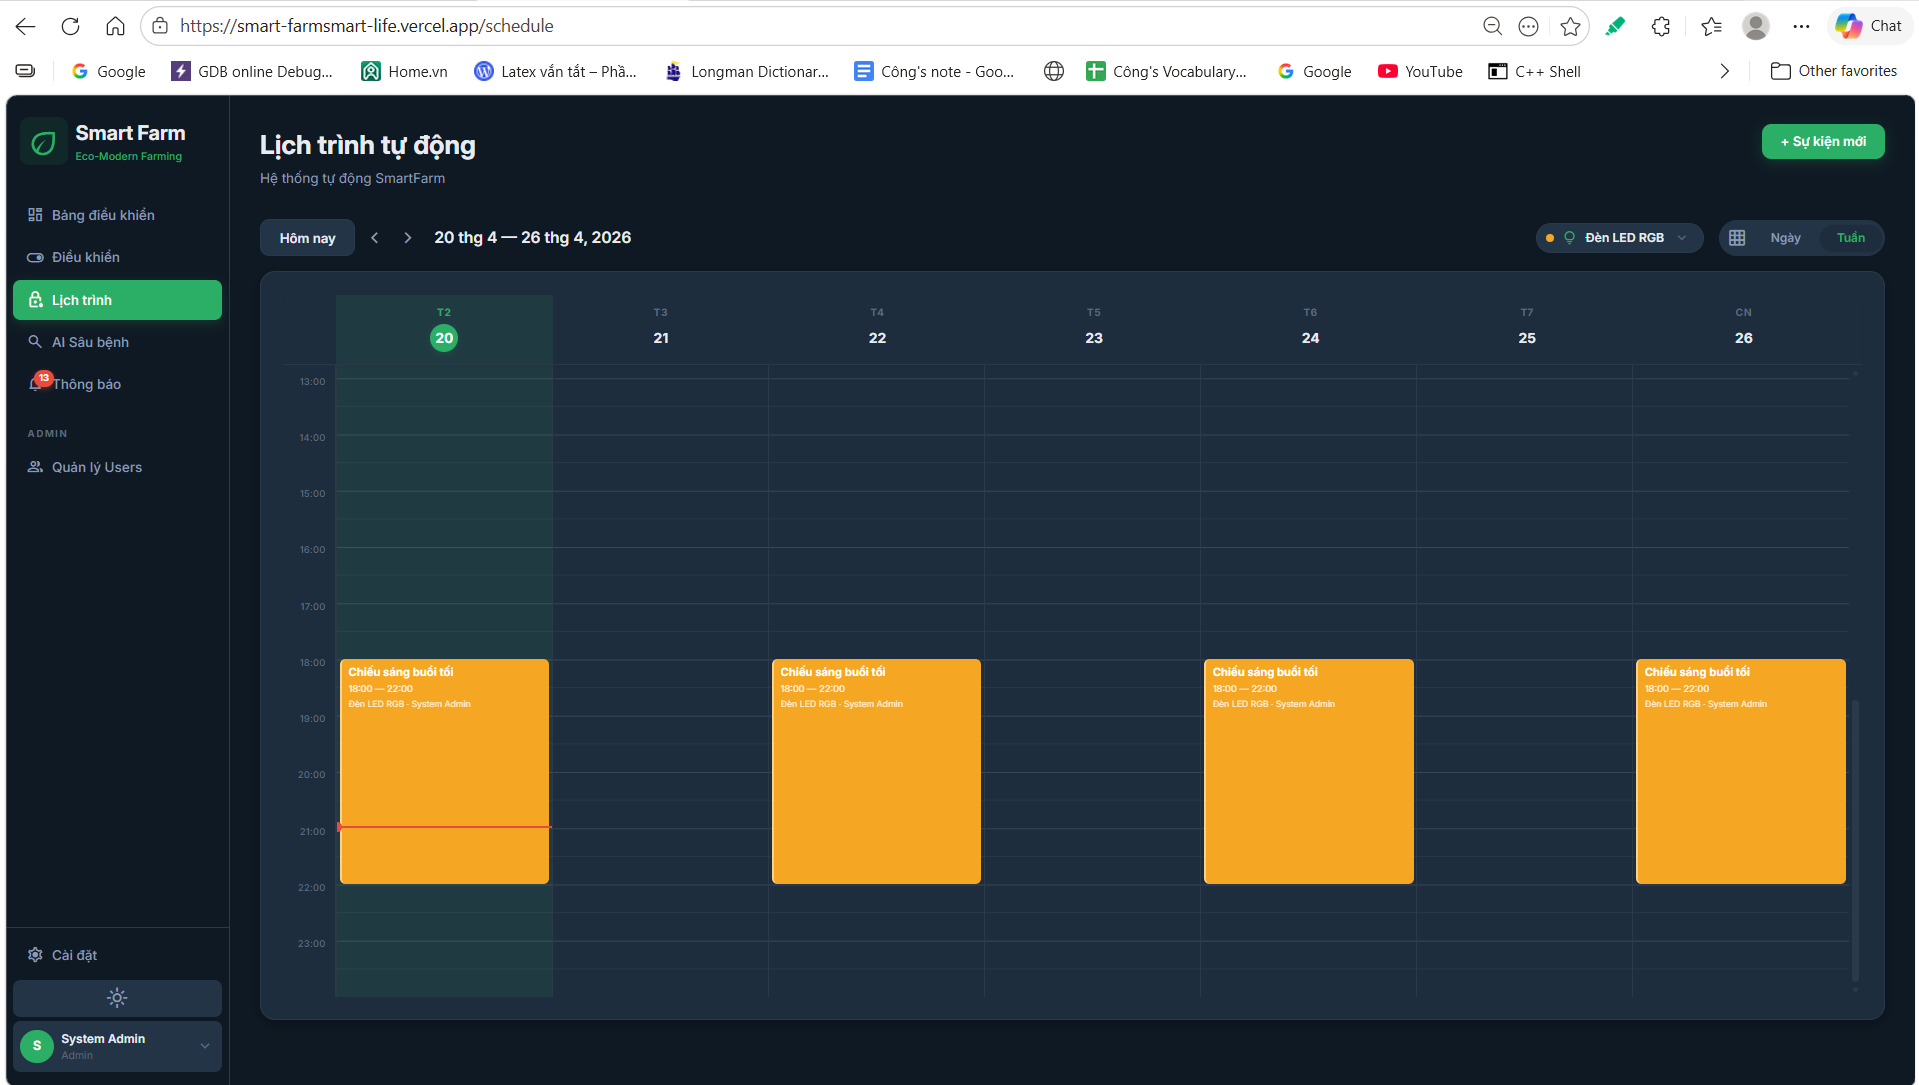
\includegraphics[width=0.8\linewidth]{./Pictures/Task_5/schedule.png}
	\caption{Giao diện phần xem lịch trình tự động hóa}
\end{figure}
\indent Có thể xem được lịch trình theo nhiều chế độ. Cụ thể là theo ngày hoặc theo tuần trên một timeline dựa vào thời gian thực. Ngoài ra, người dùng còn có thể chọn các thiết bị cần xem lịch trình (máy bơm 1, 2 hoặc đèn LED).\\
\indent Mặt khác, có thể thêm lịch trình mới bằng cách nhấn vào nút ``Sự kiện mới'' ở góc trên bên phải màn hình. Khi bấm vào nút này thì một cửa sổ nhỏ hiện lên với các thông tin mà người dùng cần phải điền để có thể thêm một lịch trình mới cho một trong các thiết bị một cách hợp lệ. Nếu lịch được thêm có ngày bắt đầu là một thời điểm trong quá khứ so với thời gian thực thì hệ thống sẽ không ghi nhận lịch trình này và báo lỗi ``lịch trình không thể bắt đầu vào một thời điểm trong quá khứ''. Mặt khác, nếu ngày kết thúc nhỏ hơn ngày bắt đầu cũng sẽ có lỗi xảy ra.\\
\indent Khi thời gian thực tới thời điểm bắt đầu một lịch trình nào đó thì hệ thống sẽ kiểm tra xem thiết bị đã hoạt động hay chưa. Nếu chưa thì hệ thống sẽ tự động khởi động (bật) thiết bị đó lên. Khi kết thúc lịch trình, nếu thiết bị đang bật thì hệ thống sẽ tắt thiết bị đó đi một cách hoàn toàn tự động.
\begin{figure}[H]
	\centering
	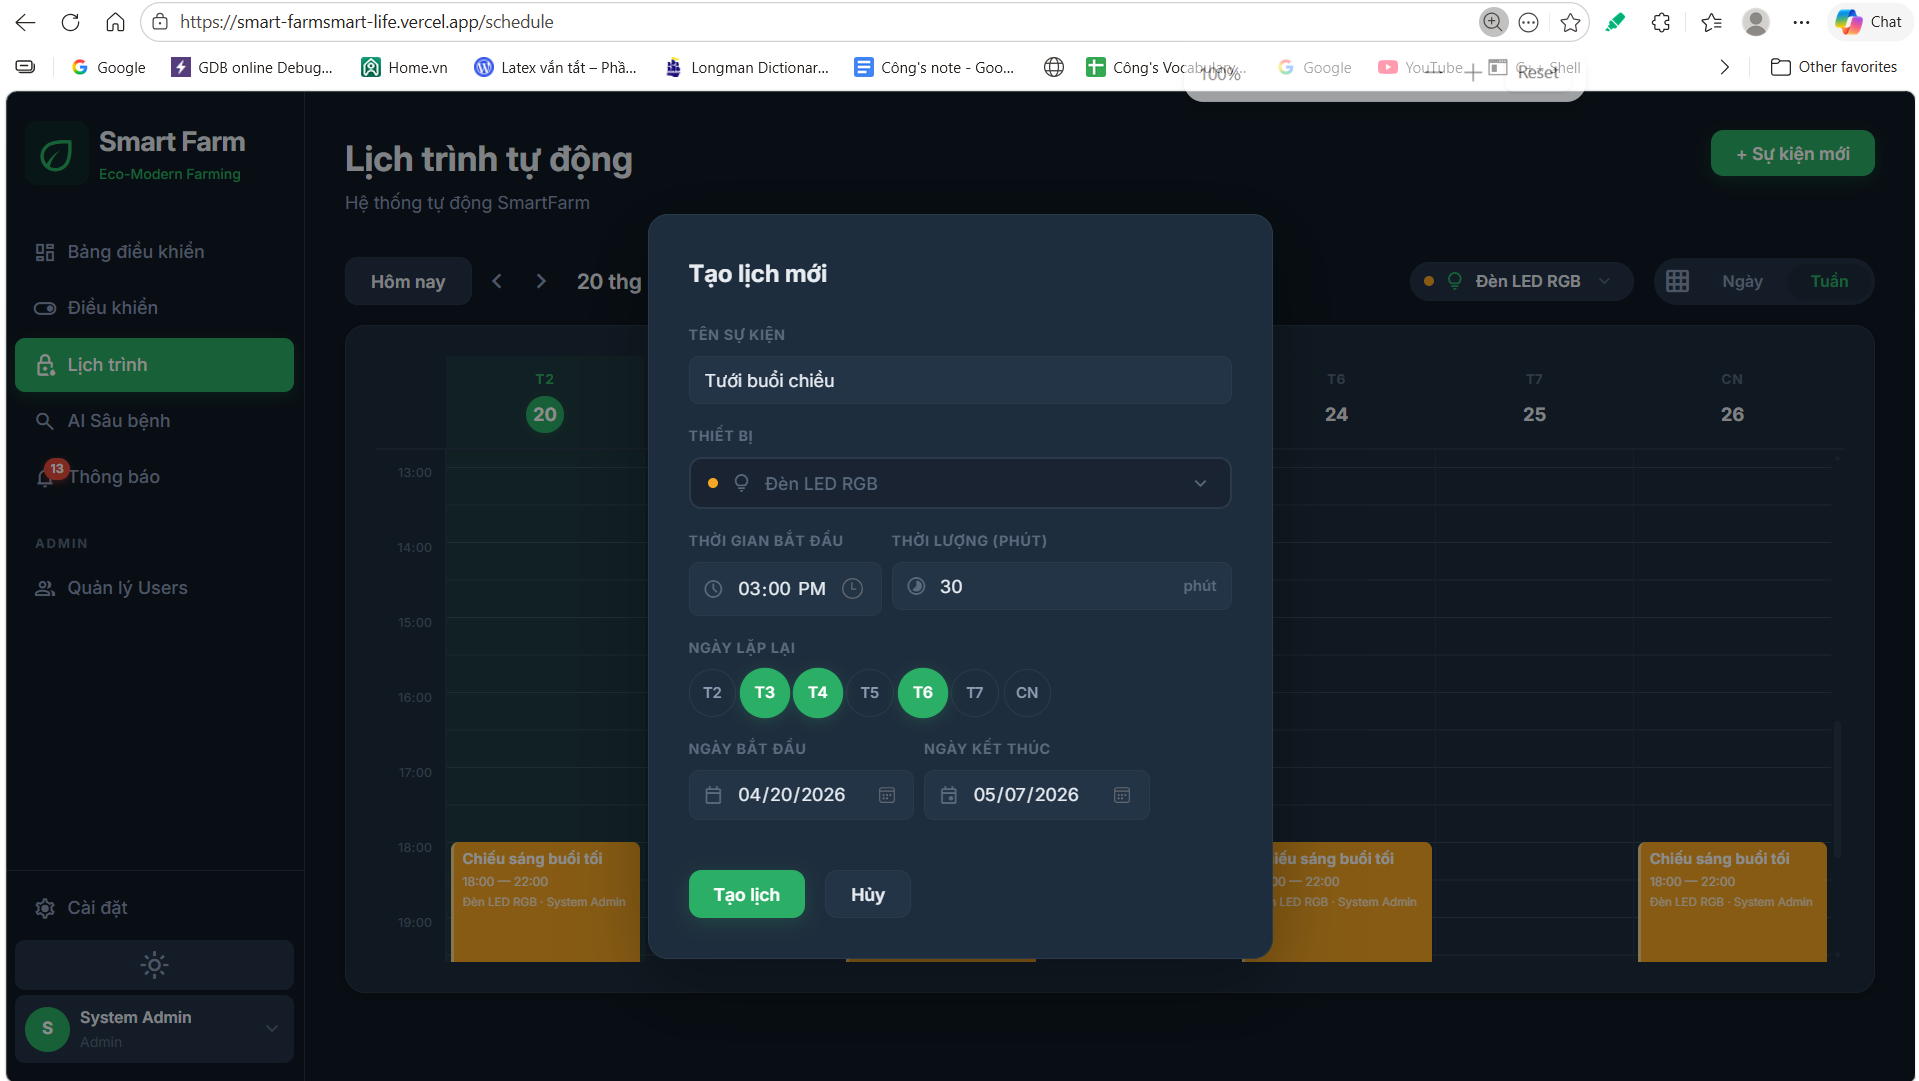
\includegraphics[width=0.8\linewidth]{./Pictures/Task_5/schedule_setup.png}
	\caption{Giao diện phần thêm lịch trình mới}
\end{figure}
\subsubsection{Giao diện hệ thống thông báo}
\indent Giao diện thông báo giúp tổng hợp và cập nhật liên tục cho người dùng nếu có cảnh báo về môi trường (như nhiệt độ bất thường, độ ẩm thấp) hoặc các sự kiện tự động hoá (đã đến giờ bật bơm). Các thông báo này đẩy qua dịch vụ Socket.IO hiển thị tự động. Nhờ giao diện trực quan, người quản trị có thể dễ dàng đánh dấu đã đọc một hay tất cả thông báo, có thể ghim/lưu (save) các cảnh báo trọng điểm, cũng như chọn xóa đi khi không cần thiết.
\begin{figure}[H]
	\centering
	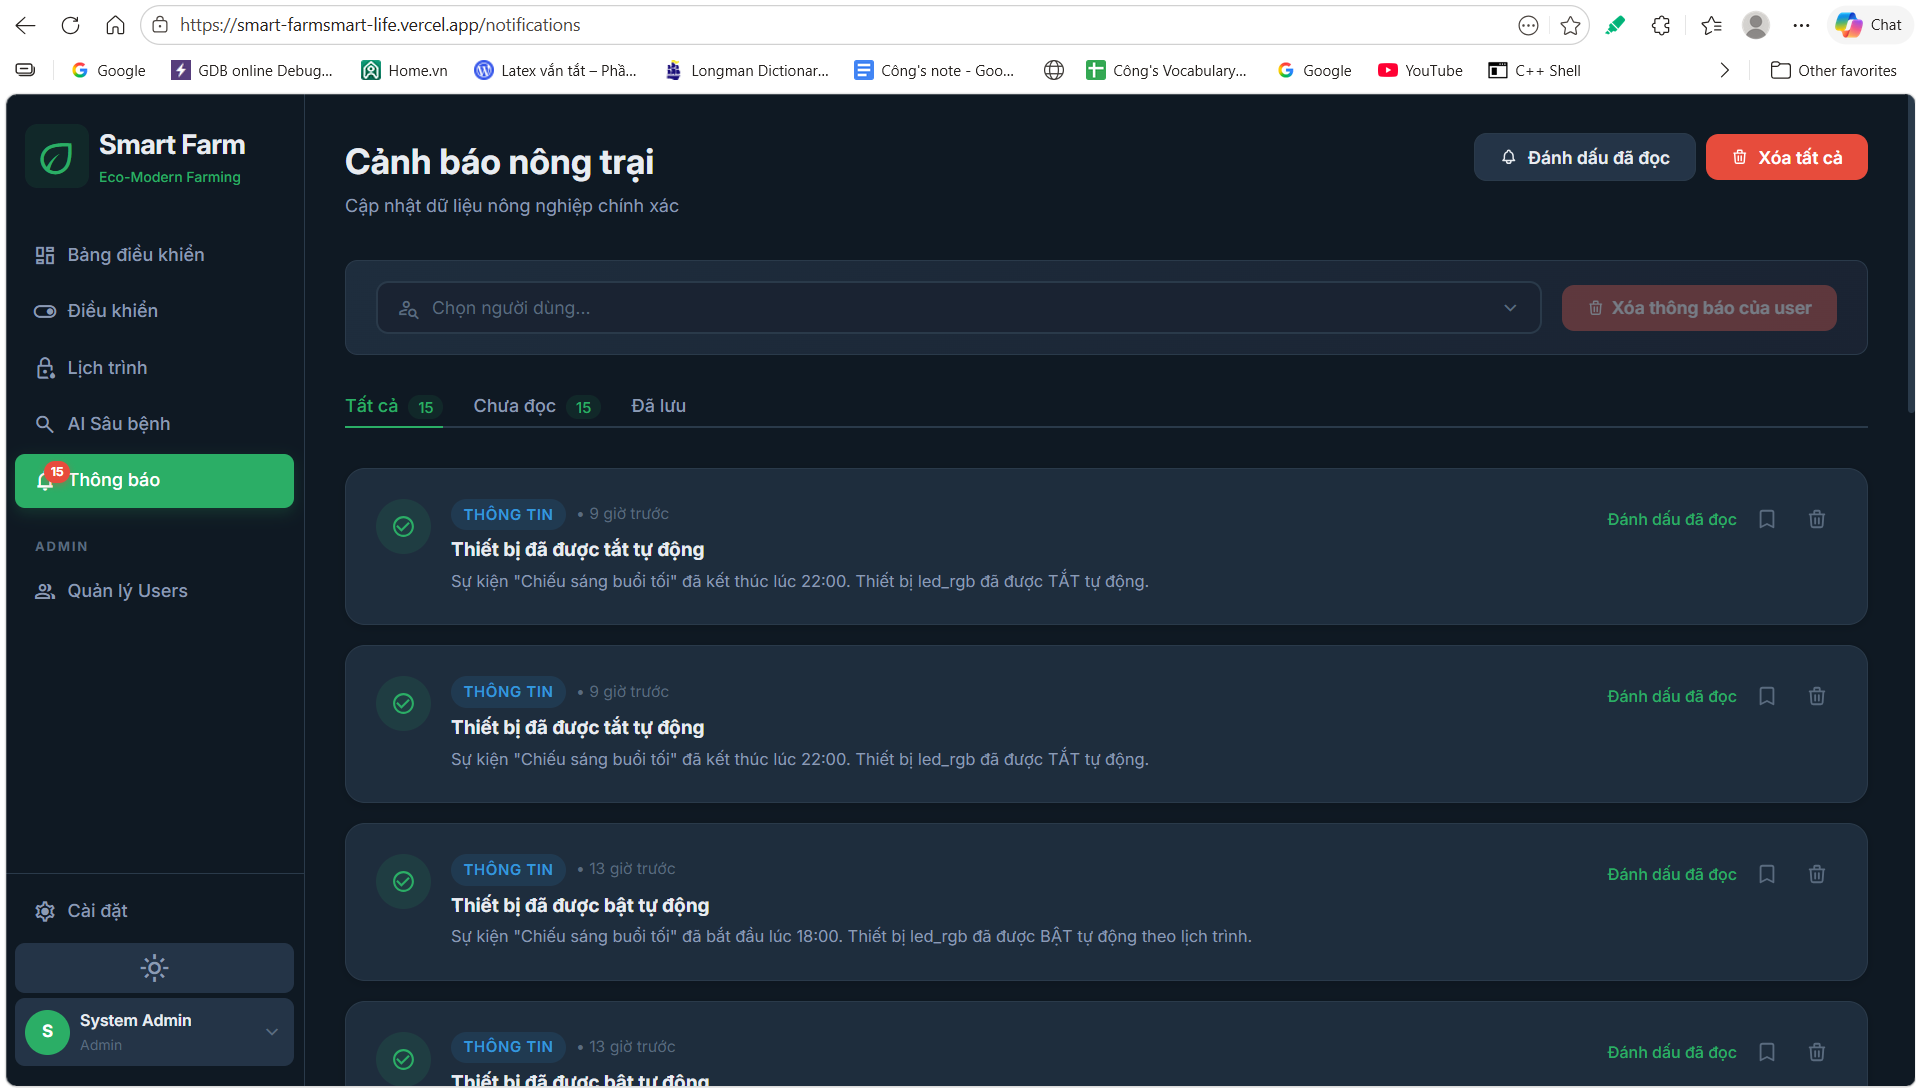
\includegraphics[width=0.9\linewidth]{./Pictures/Task_5/notification.png}
	\caption{Giao diện hệ thống thông báo báo động và giám sát}
\end{figure}

\subsection{Huấn luyện AI nhận diện lá cây bệnh}
\indent Một trong những tính năng nổi bật của SmartFarm là việc tích hợp Trí tuệ nhân tạo (AI) giúp chẩn đoán và phát hiện tình trạng sâu bệnh trên lá cây dựa vào việc phân tích và xử lý các loại hình ảnh của lá cây cà chua (png, jpg, jpeg).\\
\indent Dịch vụ AI này chia thành một microservice hoạt động độc lập bằng FastAPI, sử dụng kiến trúc mạng nơ-ron tích chập nổi bật \textbf{EfficientNet}. Thông qua việc tải ảnh lá cây bệnh lên hệ thống, tiến trình backend tại đây sẽ uỷ thác cho nền tảng AI phân tích. Chỉ trong vài giây, hệ thống trả ra dữ liệu kết quả là Tên loại bệnh, độ tự tin (confidence) của chẩn đoán mô hình, và ngay lập tức cung cấp phác đồ cách thức khắc phục (Ví dụ cắt cành sâu trị nấm,...). Đây là một ưu điểm rất lớn của hệ thống.

\begin{figure}[H]
	\centering
	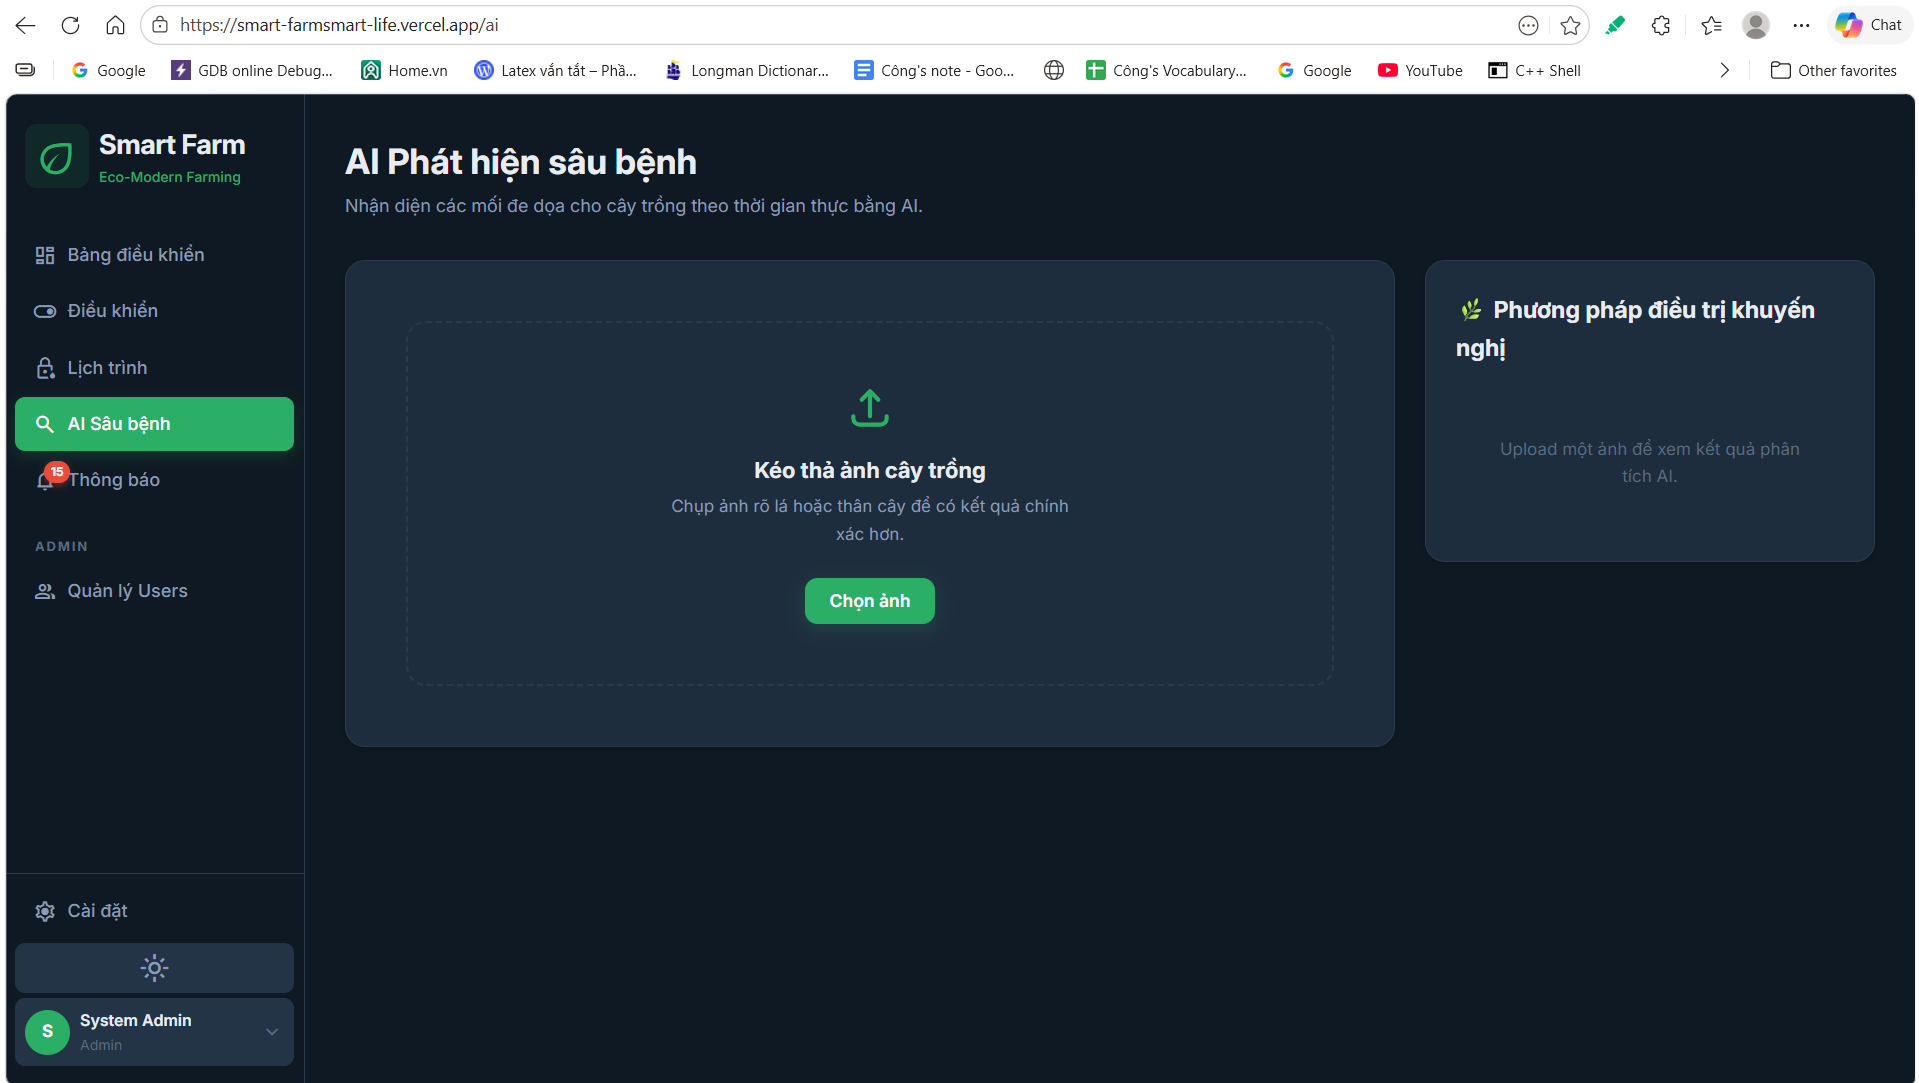
\includegraphics[width=0.9\linewidth]{./Pictures/Task_5/AI_general.png}
	\caption{Giao diện sử dụng AI chẩn đoán bệnh nông nghiệp}
\end{figure}

\indent Mô hình AI hiện tại được hệ thống chia thành 6 lớp phân loại tình trạng của rau màu (cà chua): bao gồm 1 lớp khỏe mạnh và 5 lớp tổn thương khác.
\vspace{0.2cm}
\begin{enumerate}[label=\textbf{\arabic*.}, leftmargin=1.5cm ]
	\item \textbf{Lá cà chua khỏe mạnh}
	\begin{figure}[H]
		\centering
		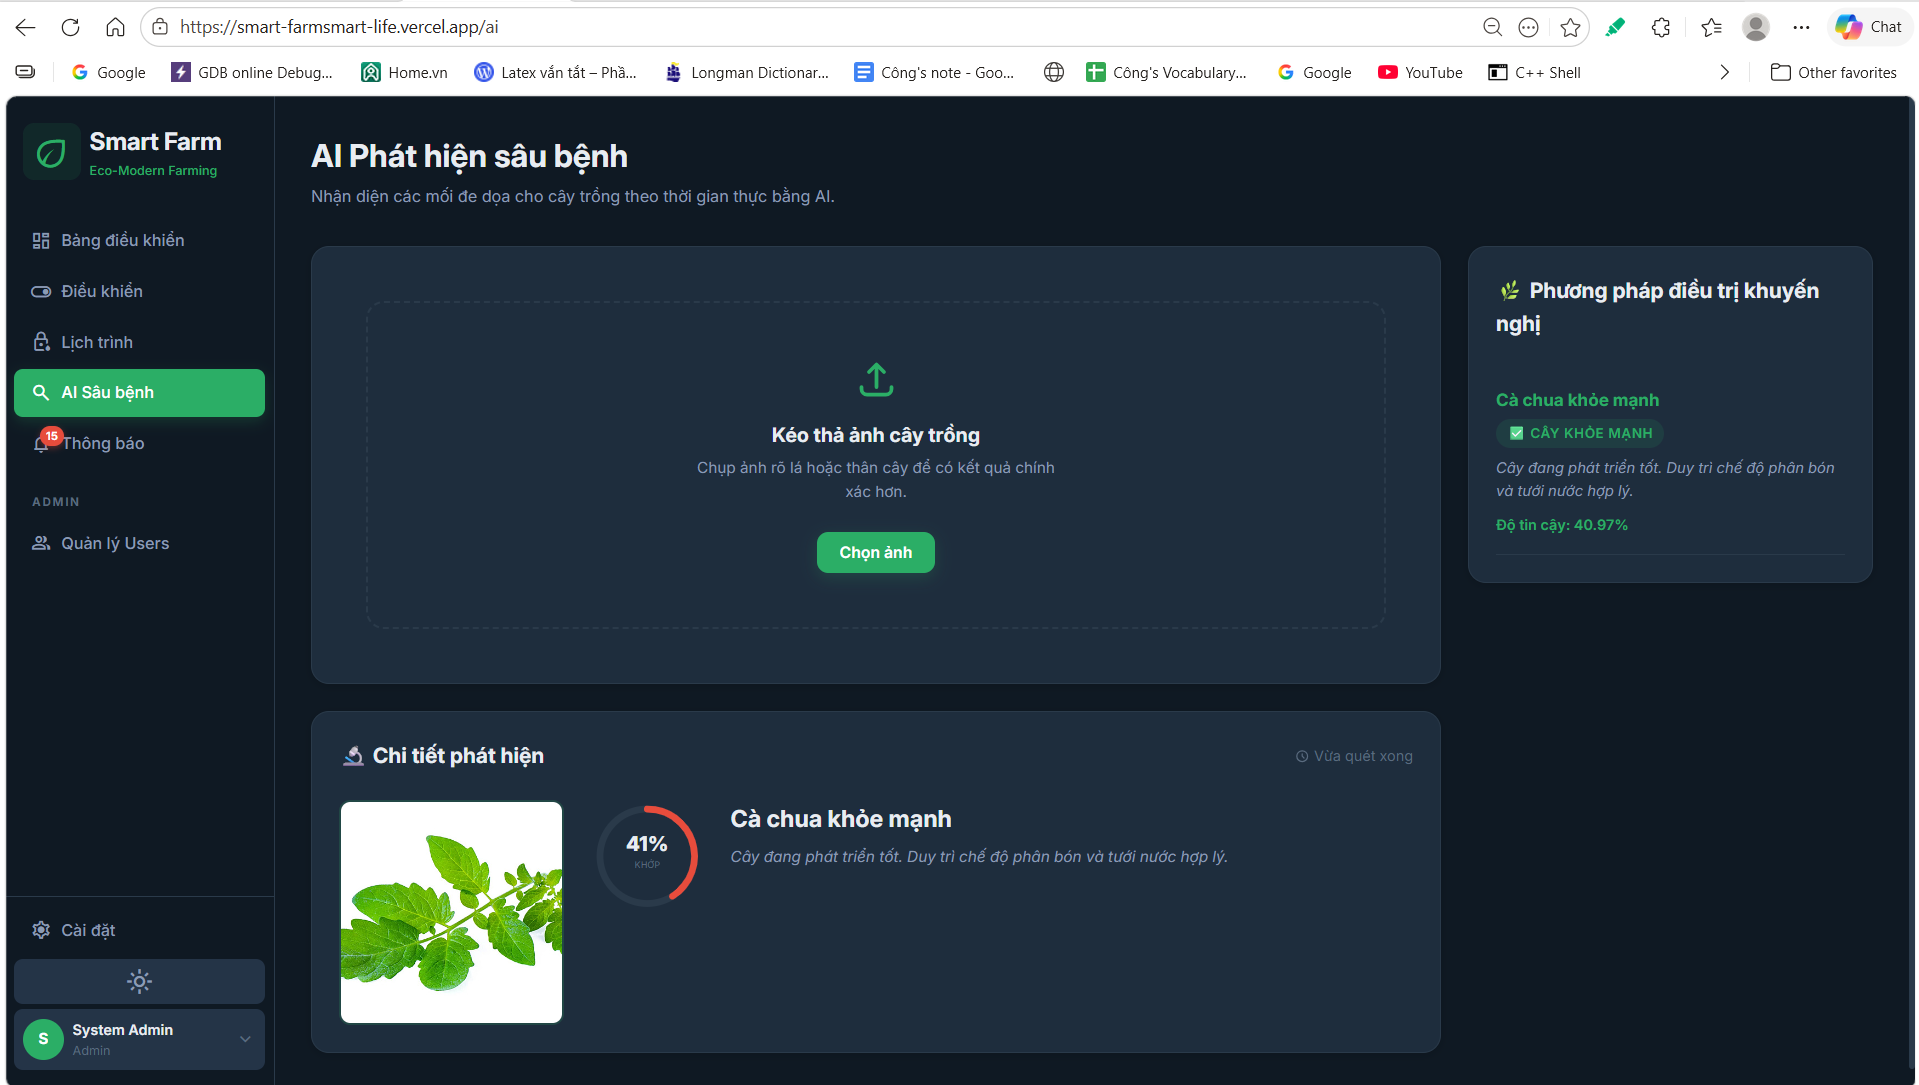
\includegraphics[width=0.8\linewidth]{./Pictures/Task_5/AI_Tomato_Healthy.png}
		\caption{Lá cà chua khoẻ mạnh (Healthy)}
	\end{figure}
	\item \textbf{Lá cà chua bị nhiễm bệnh}
	\begin{figure}[H]
		\centering
		\begin{minipage}{0.5\textwidth}
			\centering
			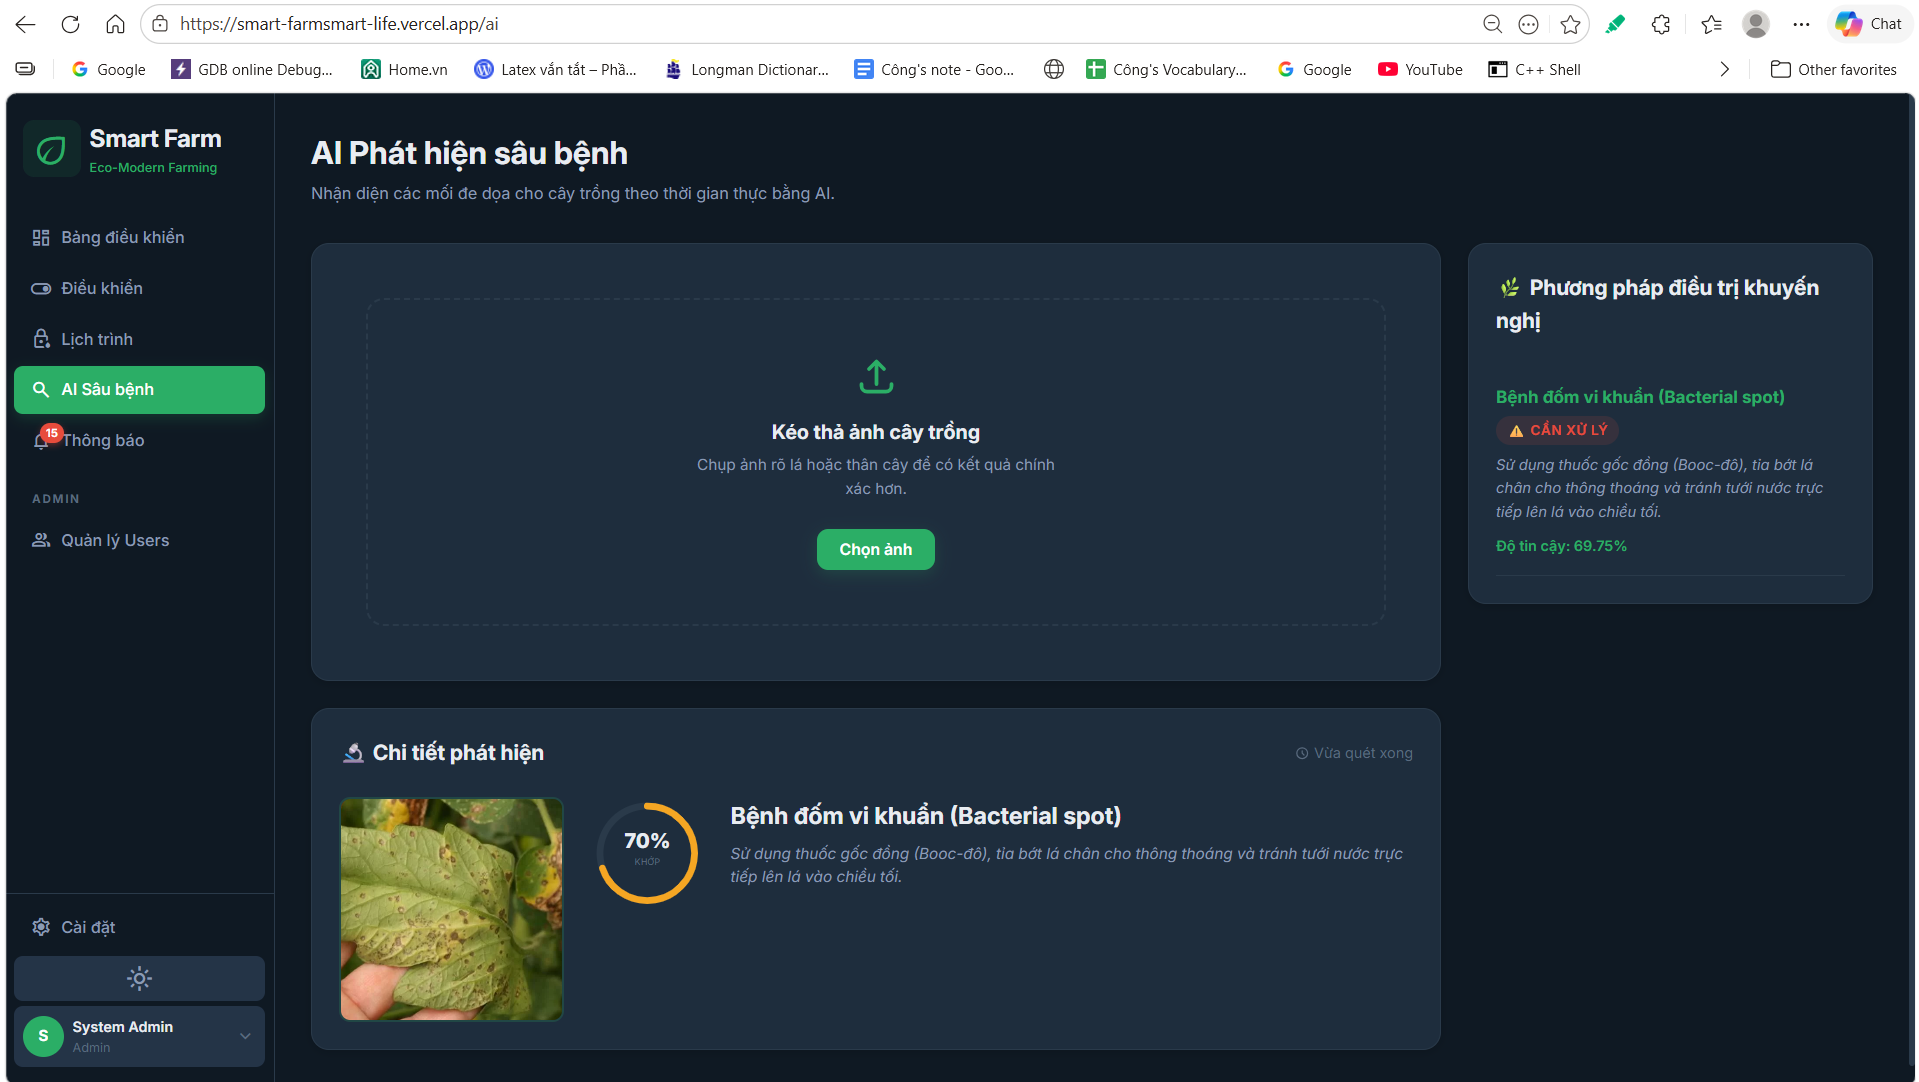
\includegraphics[width=0.95\linewidth]{./Pictures/Task_5/AI_Tomato_Bacterial_Spot.png}\\[0.1cm]
			\textit{Bệnh đốm vi khuẩn\\(Bacterial spot)}
		\end{minipage}\hfill
		\begin{minipage}{0.5\textwidth}
			\centering
			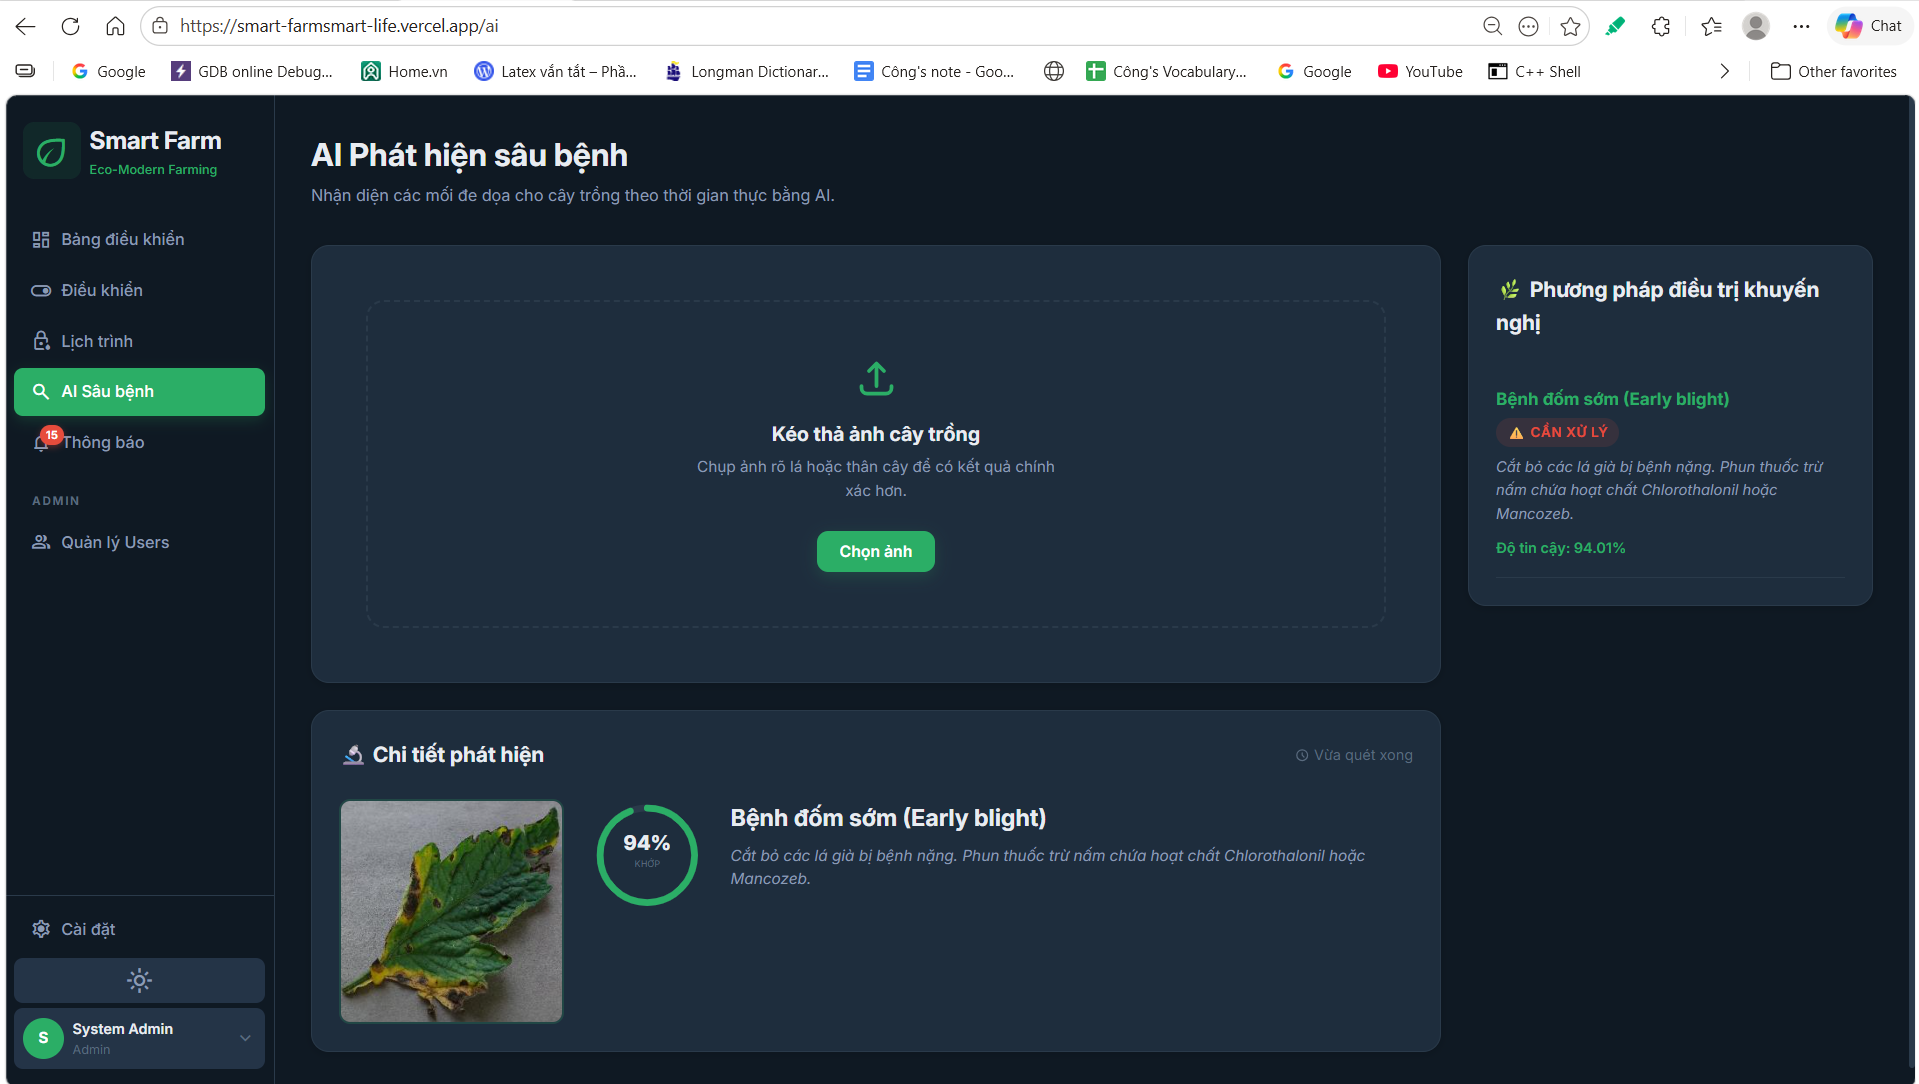
\includegraphics[width=0.95\linewidth]{./Pictures/Task_5/AI_Tomato_Early_Blight.png}\\[0.1cm]
			\textit{Bệnh đốm sớm\\(Early blight)}
		\end{minipage}
		
		\vspace{0.4cm}
		
		\begin{minipage}{0.5\textwidth}
			\centering
			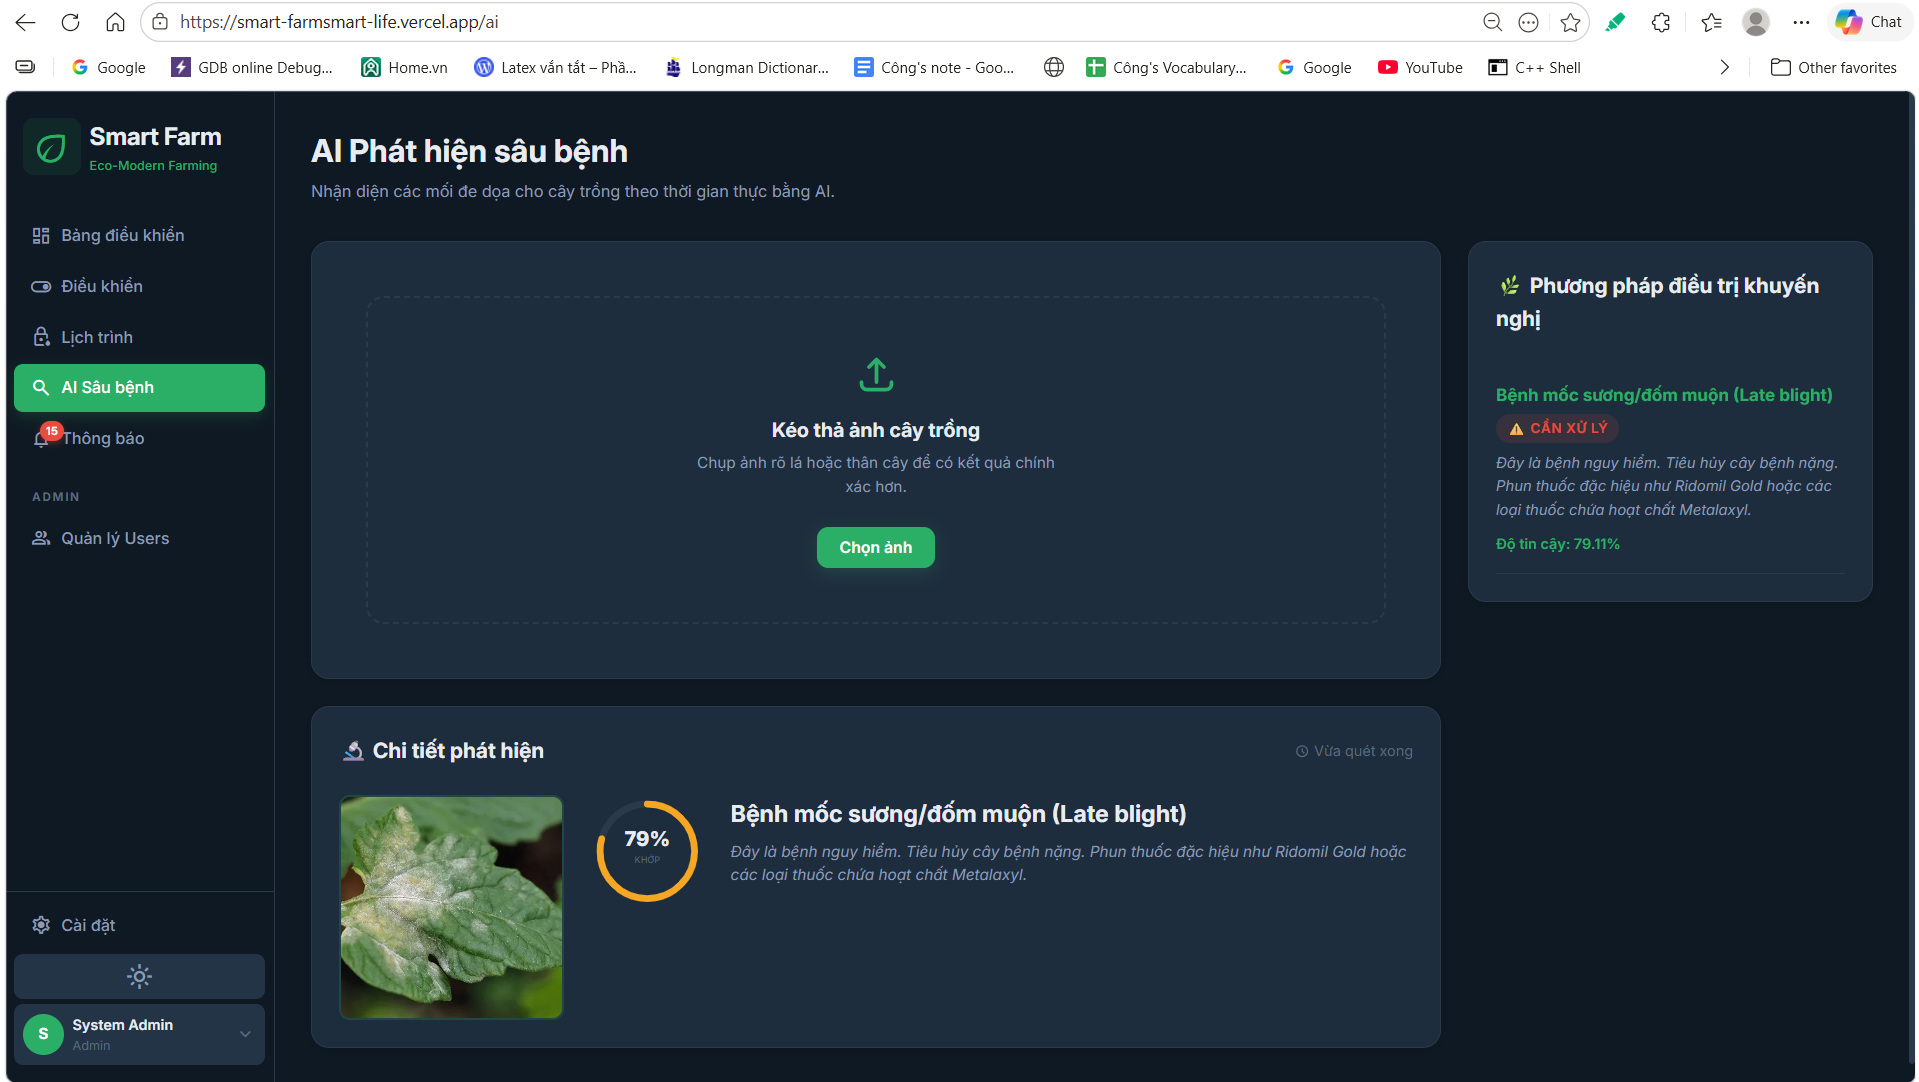
\includegraphics[width=0.95\linewidth]{./Pictures/Task_5/AI_Tomato_Late_Blight.png}\\[0.1cm]
			\textit{Bệnh mốc sương\\(Late blight)}
		\end{minipage}\hfill
		\begin{minipage}{0.5\textwidth}
			\centering
			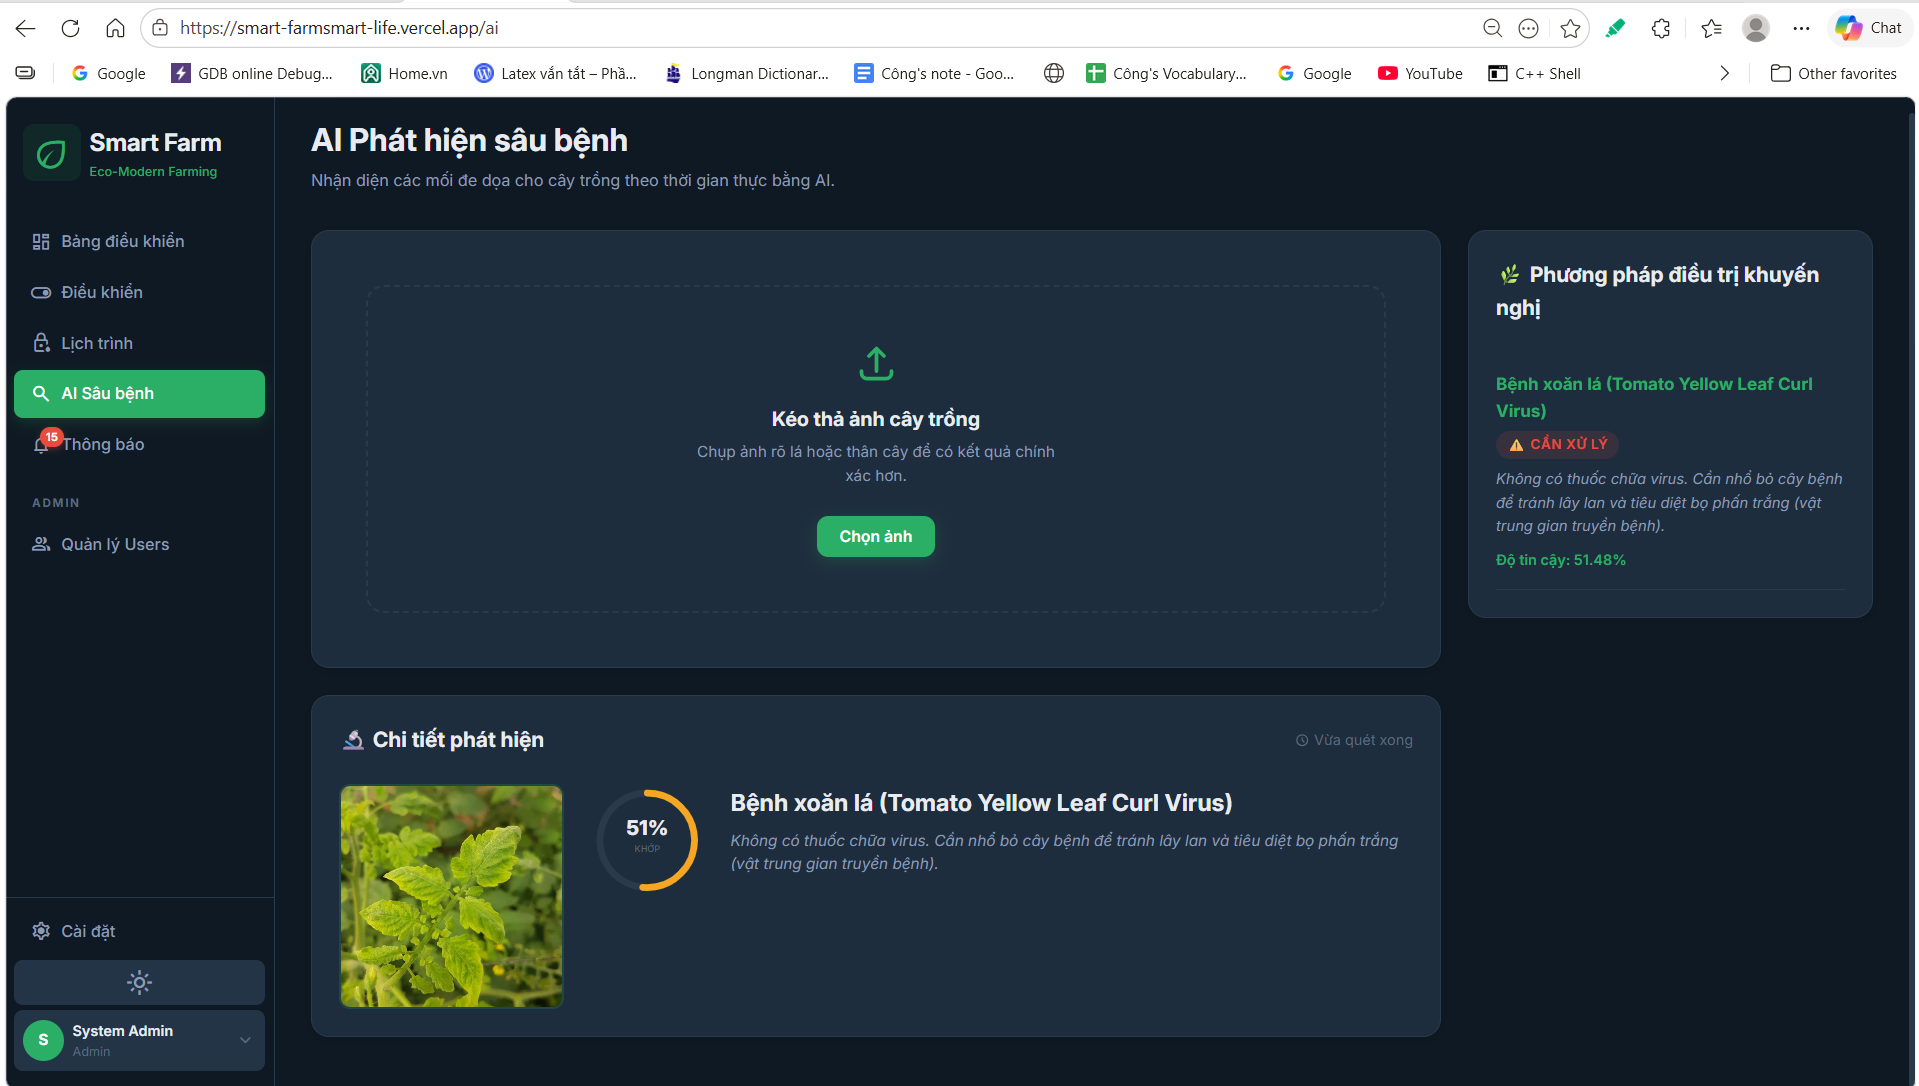
\includegraphics[width=0.95\linewidth]{./Pictures/Task_5/AI_Tomato_Yellow_Leaf_Curl_Virus.png}\\[0.1cm]
			\textit{Bệnh xoăn lá\\(Yellow Leaf Curl)}
		\end{minipage}\hfill
		\begin{minipage}{0.5\textwidth}
			\centering
			\textbf{Cùng một số bệnh lý khác được tích hợp trong mô hình (Leaf Mold,...)}
		\end{minipage}
		\caption{Các tập mẫu kết quả nhận diện trên mô hình thực tế}
	\end{figure}
\end{enumerate}
%TODO: Thêm phần mô tả về cách thức hoạt động của AI dựa trên phần xử lý hình ảnh thuộc yolofarm\server\api\main.py
